\documentclass[format=acmsmall,review=false]{acmart}
\usepackage{acm-ec-26}
\usepackage{booktabs,amsmath,graphicx}
\setcitestyle{authoryear}
\title[Who Keeps an Offer?]{Who Keeps an Offer? Predicting Partners and Choosing Shortlists in Matching Markets}
\author{Anonymous}
\newcommand{\da}{\operatorname{DA}}
\newcommand{\co}{C_{\mathrm{stab}}}
\newcommand{\allp}{C_B}
\newcommand{\HH}{H_G}
\setcopyright{none}
\begin{abstract}
A platform that recommends five options per applicant can learn to cover more historical offers and still place fewer people. We tested this prediction in two subsequent Chilean school cohorts, with frozen models and both signs specified before acquiring the data. Among 1,107,244 applicants, giving the predictor access to reported rank covered 2,493 additional initial offers, including 2,244 that families explicitly accepted, yet placed 985 fewer applicants under replayed deferred acceptance. The primary comparison with uniform lists favors learning on both outcomes. We then ask what a designer can guarantee. Before matching, a min-cost flow computes the least predicted coverage a platform must sacrifice to accommodate a given number of simultaneous assignments. For 189,399 university applicants, increasing this feasible number by 1,311 produced only 19 additional DA placements. After observing tentative offers, one quota-preserving referral per selected applicant can instead realize a maximum extension of the original contracts without worsening any current recipient's assignment. With 21,061 vacant university seats, only 160 unmatched applicants had listed a reachable program; the exact safe extension placed 147, falling to four if referrals had to be among the applicant's first five choices. Rental simulations and bilateral preference data illustrate how scarcity, coordination and the choice of comparator affect these results. Policy effects hold reported preferences fixed; historical offers and acceptances are observed.
\end{abstract}
\begin{document}
\begin{titlepage}
\maketitle
\thispagestyle{empty}
\end{titlepage}

\section{Introduction}
A school platform recommends five programs to each family. Its engineers find a way to show more families the program they would eventually be offered. Should they change the recommendations? All five programs are also seats for which other families can apply. To answer, one must count people left without a place, including the people whose recommendations never changed.

We study this question in systems that clear shortlists by applicant-proposing deferred acceptance (DA). A natural learning target is the program an applicant would obtain if every submitted option remained visible. This target has a precise justification. If a display omits $r$ original matched pairs, no more than $r$ originally matched applicants can become unmatched; the people who lose can differ from those whose own partners were omitted. We relate predictive loss to this bound and test the resulting recommender in markets built from New York rental advertisements and survey households. Learning roughly doubles full-market partner recovery relative to uniform lists in ordinary markets, yet fewer renters obtain a placement. Most lower-income renters in those markets have no affordable unit to begin with. We keep them in the denominator and examine a deliberately enriched supply scenario separately.

Chilean school and university admissions provide a different test. Students submit preference orders, and public records identify initial offers. Against uniform lists, the primary learned rankings in both systems improve both coverage and placement. But giving an offer predictor the order of a student's choices, in addition to the set of programs, improves coverage at a cost to placement. After seeing this comparison in two school years, we fixed the 2019 models and specified both signs before acquiring two later national cohorts. In each new year, the rank-informed rule covered more historical offers and placed fewer pupils under DA. In the university cohort, the same conclusion held for observed enrollment destinations, including when the model was trained on registrations. Only list coverage is directly measured on these historical outcomes. A placement under changed menus requires a counterfactual replay.

The design question depends on timing. Before any offer exists, how much prediction accuracy would a platform have to give up to accommodate $r$ simultaneous assignments? We give an exact reduction to a minimum-cost capacitated assignment. In university admissions, almost all predicted coverage can coexist with the maximum number of feasible assignments. DA nonetheless realizes little of the extra capacity. Its competition and priority rules still apply to the new lists.

After tentative offers exist, the platform can instead ask which unmatched people can use a remaining seat. We prove the largest number who can be added while keeping every provisional contract available in a stable allocation. One new recommendation per selected applicant suffices, keeping each list within quota, and DA gives every original recipient an assignment weakly preferred to their tentative one. The 2026 university replay has 21,061 empty seats but just 160 unmatched students who listed a reachable program. It is possible to place 147 of them. If the service restricts itself to the student's five highest submitted choices, only four additional placements are possible. This finding describes the limits of curating previously reported options. Finding new options that applicants would actually want is a different intervention.

\section{The market and related work}
Let $B$ be applicants and $S$ one-capacity listings. Each vertex strictly ranks its neighbors in the bipartite feasibility graph $E$ above the outside option $\bot$. For a displayed graph $D\subseteq E$, applicants propose down their rankings restricted to $D$; each listing retains its favorite proposal so far. Write $\da(D)$ for the final matching and $M(i)$ for $i$'s partner. A pair blocks on $E$ when both parties strictly prefer each other to their assigned partners. DA is stable on the displayed graph and applicant-optimal among its stable matchings \citep{gale1962}. In strict one-to-one markets all stable matchings of a \emph{fixed} graph have the same matched participants \citep{galesoto,roth1986}. Whenever visibility changes, our outcome is the matching returned by DA on the new graph. We rank unmatched below every feasible option.

\citet{menus} describe DA in terms of the menu an applicant faces when others' reports are fixed. \citet{papai} studies when a singleton report attains an object. We use these results to attach an external consequence to each attainable option: which other applicant loses a placement. The consistency of stable allocations under removal of matched pairs is classical \citep{sasaki}. Our coalition result uses this consistency to recover identities after a shortlist change, and the rollout experiment measures the discrepancy from adding single-applicant effects. Competition in two-sided recommendation and interference in platform experiments are already well established \citep{rankings,johari2022}. Our comparisons use explicitly paired assignments under the entire recommendation policy.

Short proposal lists can retain good partners under particular preference models \citep{shortlists}. Other work restricts the pairs allowed to block \citep{askalidis2013} or the pairs permitted in a stable assignment \citep{cseh2016restricted}. Here feasibility, display and full-market stability are distinct. Our burden bounds use threshold costs, in the spirit of optimization of order statistics and model-compatibility tests \citep{gorski2009,ekeland2010}. We use known matching and polyhedral methods to produce sharp finite-market welfare comparisons. Our audit problem is also related to costly expansions of compatibility \citep{facilitate}, input-error mitigation after DA \citep{postmatch}, and incremental matching \citep{incremental}.

Recommendations under partial information have a long history in matching markets. \citet{signals} use informative signals and match recommendations to economize on communication. \citet{pruned} use predicted partner ranks to truncate a side's ordered preferences and analyze full-market stability and proposal counts. Our target is who loses a placement after arbitrary feasible edges are hidden, including people whose own preferences or displays stay fixed. \citet{smartplatforms} document how informing Chilean families about admission risk can change search and improve actual placement. We hold reports fixed to isolate a different question: how two shortlists of the same size compete for seats. \citet{tworound} minimize school reassignments after a market changes. Our decision variable is the list shown to a competitor before DA runs again. \citet{reallocation} study protection of initial endowments through ownership-adjusted priorities. Our certificate uses the original priorities on a changed display. For a comparison with an implemented recommendation algorithm, we reproduce and adapt \citet{rankings}, keeping separate their interview outcome and our unit-capacity allocation.

\paragraph{A displacement fact used below.} Fix a group of applicants whose lists do not change. In a stable assignment, remove all outsiders along with the seats they occupy. The remaining applicants are stably matched in the residual market: a blocking pair there would also block the original assignment. The set of matched applicants is invariant across stable assignments on that residual graph. Removing one available seat can displace at most one incumbent; this follows by adding the seat back using listing-proposing DA. Appendix~\ref{sec:menu} proves this claim and identifies the displaced applicant when one competitor edits a list.
\citet{sekiya2026} limit exposure on the receiving side of a dating platform and measure changes in mutual contacts in a field experiment. Our capacity requirement asks how many different applicants the displayed graph can assign simultaneously. Our downstream outcome is a priority-respecting allocation. \citet{lepesure} studies guaranteed recommendations of previously unlisted schools using a targeted vacancy market in Chile. Our after-offer result uses omitted options already declared acceptable and gives an exact bound for one fixed-quota substitution per entrant.
\section{What should a shortlist model predict?}\label{sec:prediction}
A renter's favorite five units can all go to someone else. If the platform knows the distribution of preferences but observes only market attributes $X$, there is another possible prediction target. Let $M=\da(E)$ be the allocation that would result if all feasible listings were visible. Let
\[
   p_{ij}(X)=\Pr\{M(i)=j\mid X\},\qquad j\in E(i)\cup\{\bot\}.
\]
These probabilities include the possibility of getting no offer. They incorporate competition from other renters for the same listings. In the housing application $M$ is a simulation label. There are no observed full-information allocations.

\begin{theorem}[Placements lost when partners are omitted]\label{thm:omission}
Take any stable matching $M$ on $E$, any display $D\subseteq E$, and any matching $N$ stable on $D$ with preferences restricted from $E$. Let $H=\{i:M(i)\ne\bot,\ (i,M(i))\notin D\}$, and let $K$ and $T$ be the real listings occupied by $H$ in $M$ and $N$, respectively. Both the number of applicants who go from matched to unmatched and the number who go from unmatched to matched are at most $|H|-|K\cap T|$. The bound $|H|$ on losses can be tight even for disjoint applicant--listing pairs.
\end{theorem}
\begin{proof}
Put $I=B\setminus H$. Remove $H$ and $K$ from $M$. Every surviving assignment is visible in $D$ by definition of $H$. Its restriction is stable for the remaining participants on $D$, since a block there would block $M$ on $E$. Thus the initially matched members of $I$ are $F(S\setminus K)$, using the incumbent lists on $D$. Deleting $H$ and $T$ from $N$ gives the final matched incumbents $F(S\setminus T)$. By Theorem~\ref{thm:occupied-seats}, at most $|T\setminus K|$ members of $I$ lose a placement. Among $H$, all were matched initially and exactly $|H|-|T|$ lose. Their sum is at most $|H|-|K\cap T|$. Only incumbents can gain, and at most $|K\setminus T|$ do so. Here $|K|=|H|$. Deleting the sole edge of each of $r$ isolated pairs gives $r$ losses.
\end{proof}

\paragraph{A learning objective with an assignment interpretation.}
For any displayed set of $k_i$ feasible listings per renter, the expected omission count given $X$ is
\[
 \mathbb E[|H|\mid X]=\sum_i\left[1-p_{i\bot}(X)-\sum_{j\in D(i)}p_{ij}(X)\right].
\]
In each row select the $k_i$ highest $p_{ij}$. This minimizes the expected coarse upper bound on gross losses even though the assignment outcomes depend on the whole display. The same argument permits fixed weights on omitted partners, but such weights by themselves give no group-specific loss bound: the renter who loses can be someone whose own partner stayed visible. A more accurate model of $p_i$ has a quantitative interpretation. For estimated probabilities $s_i$ on listings and the outside option, the excess expected omissions of its top-$k_i$ rule over the Bayes rule are at most $\sum_i\sqrt{2D_{\mathrm{KL}}(p_i\Vert s_i)}$. Indeed, the $s_i$-optimal set has at least the estimated mass of the $p_i$-optimal set. Replacing each of these two estimated masses by its true mass costs at most one total-variation distance, then Pinsker's inequality gives the stated bound. Categorical log loss encourages precisely this conditional-distribution fit. The theorem does not order policies by total placements or by rent burden.

For example, the first renter ranks $x$ above $y$, the second can rent only $y$, and $y$ gives the first renter priority. Under full exposure both are placed. Show the first renter only $y$ and the second loses their sole option to the first. The omitted partner and the lost placement belong to different people. We checked the bound independently on 421,200 preference/display combinations across $2\times2$, $2\times3$ and $3\times2$ markets, and 100,000 random instances with up to eight participants per side. Both gross directions were checked in every instance.

\paragraph{Protecting tentative recipients when competitors change lists.}
Construct a bipartite graph from competing applicants to the units held by the group to be protected. Include a proposed application to a held unit if its program might rank the competitor above the current holder; if priorities are unknown, keep all such edges. A maximum matching in this graph bounds how many originally matched applicants can become unmatched (Theorem~\ref{thm:threat}). At zero such edges, each protected applicant receives an option weakly preferred to their tentative assignment under applicant-proposing DA. To see why, consider the first time a fixed applicant is rejected by their initial program. An outsider cannot cause the rejection. A different fixed applicant preferred their own tentative assignment to getting this unit, by initial stability. They could not have proposed here before losing their own assignment, contradicting the choice of first rejection. When a competing applicant cannot fill their quota without adding a threat, keep their original list and protect their tentative unit too. Iterate until all remaining applicants can fill their quotas. Appendix~\ref{app:protect-detail} gives the sharp bound and algorithm.
\section{Rental markets and experimental design}
We use 2020--24 American Community Survey (ACS) Public Use Microdata Sample household records and FirstMover monthly rental advertisements at first appearance \citep{acs,firstmover}. Incomes and prices are expressed in July 2026 dollars using national CPI-U \citep{cpi}. A lower-income household earns at most the survey-weighted median income of all NYC cash renters (\$64,435 in 2024 dollars). A unit must be in the same borough, cost at most 40\% of monthly household income, and meet a bedroom requirement of $\max(0,\lceil h/2\rceil-1)$ capped at eight for household size $h$. The maximum monthly rent at the group cutoff is \$2,286.

The calibrated study draws from 7,193 recent-mover households and from June--August 2026 arrival catalogues. Requiring valid listing fields, checking geography, filtering nominal asks to \$800--20,000 and deduplicating within month left 66,043 NYC listing records from 72,542 raw arrivals. Staten Island had 26, 26 and 20 listings and could not supply a draw of 64. The Bronx, Brooklyn, Manhattan and Queens account for 97.95\% of the intended recent-mover geographic weight. Outcomes are simulated separately within borough-month. A household or listing may recur across draws. The archive includes the construction rules and losses to cleaning.

\paragraph{Two protocols for drawing markets.}
Ordinary markets draw 64 renter instances with replacement using household weights and 64 distinct listings uniformly. In enriched markets, 32 listings come from an affordability band and 32 from above it. The band ends at the survey-weighted 75th percentile of budgets among lower-income donors who can afford at least one listing in the entire borough-month catalogue and meet its bedroom requirement. We then sample 32 lower-income renters who have an eligible unit in the \emph{drawn} inventory and 32 higher-income renters from their ordinary frame, using survey weights within each pool. The enriched sample is a conditional stress test. In ordinary pilot markets 86.96\% of lower-income instances had no option after geographic standardization.

\paragraph{Holding tastes fixed while altering advice.}
Let $b$'s monthly budget be $c_b$, $r_s$ the asking rent, $Q_s$ the mean of standardized physical attributes (log area and bathrooms), $a_{bs}$ spare bedrooms capped at two, and $d_{bs}$ distance in kilometers from the centroid of the renter's area. The observable score with price penalty $w$ is
\[
   v_{bs}(w)=Q_s-wr_s/c_b+0.5a_{bs}-0.5d_{bs}/5 .
\]
Renter utility on eligible pairs is $v_{bs}(w_p)+0.5\xi_s+\sigma\epsilon_{bs}$, with independent standard normal listing and pair shocks. Listings rank by $2.5\min\{I_b/(12r_s),40/12\}$ plus standard normal pair noise, where $I_b$ is annual income. We use deterministic tie breaking. In the nine-point calibration grid $w_p\in\{1,2,4\}$ and $\sigma\in\{0.50,0.75,1.25\}$, the smallest average absolute error across lower/higher rent-burden quartiles was at $(4,0.50)$ (Section~\ref{sec:burden}).

Policy U samples the quota uniformly from eligible listings. Policy $T_w$ returns the highest-scoring eligible listings under $v_{bs}(w)$. Each arm shows $\min(5,d)$ options to a renter with $d$ feasible units, or $\lceil0.4d\rceil$ in the proportional-quota exercise. The higher-income-only interventions hold the latent rankings, listings and lower-income lists fixed; only higher-income recommendations change. A separate sensitivity varies the behavioral model itself. The outcomes follow from visible applicant-proposing DA. In this model all feasible opportunities are preferred to being unmatched. The simulation does not model endogenous rents, search timing or acceptance of a binding contract.

\paragraph{Estimands and independent variation.}
Within each borough-month, sum matched lower-income renters and divide by the sum of all lower-income renters, including those with no option. Average cell rates using common renormalized borough weights and equal month weights. Each seed block contains an entire set of markets; bootstrap resampling keeps that block and its paired interventions intact. A change of one percentage point means one additional placement per hundred lower-income instances under these weights. Our intervals quantify simulation variability conditional on these catalogues, donor pool and ranking assumptions. The burden exercise instead pools matched renters across calibration draws because its target is the fitted distribution among placements.

\paragraph{Research methods and AI assistance.}
The team supplied the intermediation question, public-data pipeline and pilot protocol. OpenAI Codex assisted with formulating and proving extensions, developing the controlled counterfactuals, implementing solvers and simulation replays, analyzing outputs, preparing figures and drafting the text. The underlying housing observations come from the stated public sources. The trained rankers used numerical housing features. The AI-assisted work also includes their implementation, a published benchmark replication, the proofs about displacement and the observed-preference studies using the sources in Section~\ref{sec:field}. Our checks include independently implemented DA and optimization routines, explicit feasible assignments, exhaustive small-market comparisons and archived block-level outcomes. These are computational checks; the study does not rely on observed renter responses.


\section{Learning and testing five-listing recommendations}\label{sec:learned}
We train on 1,920 summer markets (122,880 renter outcomes) and select epochs on a separate 384. Each label is a partner or the outside option in full-exposure DA. Each feasible edge has five features: rent relative to the budget, spare bedrooms, distance, listing quality and the capped income-to-annual-rent ratio. The network sees eligibility and these features. Neither actual simulated priority draws nor renter or listing identifiers enter its predictions. The score for a listing can depend on the other renters competing for it. Two rounds of message passing average the feasible edge representations for each renter and each listing; separate heads score the edge and the outside option. We minimize cross-entropy over feasible listings and the outside option and average the predictions from three validation-selected fits. The basic pointwise comparison removes competition messages. Appendix~\ref{app:ai} describes the architecture, capacity control and precision checks.

We froze all policies and tested on 48 new summer blocks and 48 winter blocks (2,304 markets). For each market we score the same feasible apartments and run DA with the same hidden preferences under every policy. We compare uniform sampling, the transparent score $T_4$, and a congestion-aware ranking from \citet{rankings}. In its original interview setting we reproduced the ordering of the three methods using the authors' code; our rental adaptation optimizes their two-sided surrogate under the housing quota (Appendix~\ref{app:su-replication}). For an assignment-aware comparison, take a maximum-cardinality feasible matching, breaking ties by greatest total rescaled score. Put its assigned edge on each matched renter's list and fill the remaining slots by score. We call this an \emph{anchor}. It reserves a display slot, with no obligation on either party to accept that unit. When only higher-income lists change, compute anchors on the full market and replace the lower-income lists by their original uniform ones.

\begin{figure}[ht]\centering
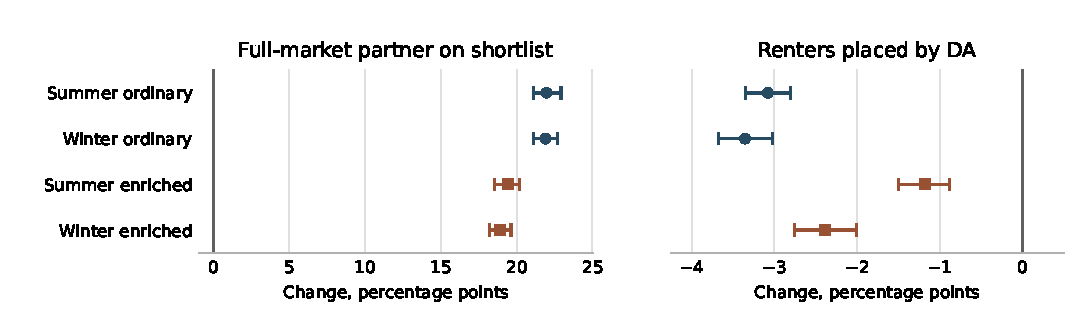
\includegraphics[width=.97\linewidth]{figures/accuracy_placement.pdf}
\caption{Replacing uniform shortlists with the contextual model for everyone. In each panel the zero line means that the two policies agree on the average rate. Whiskers are paired pointwise 95\% intervals over 48 seed blocks. Partner recovery uses renters matched under full exposure; placement uses all renters. Absolute levels and eight policies appear in Table~\ref{tab:ai}.}
\Description{In each of four panels the contextual model raises partner recovery by about twenty percentage points and reduces placement by one to four percentage points.}\label{fig:predict}\end{figure}

\paragraph{Predicting the full-market partner.}
In ordinary summer markets, the contextual rule displayed the full-market partner for 39.55\% of matched renters, against 17.58\% for uniform and 36.05\% for the pointwise model. Its advantage over pointwise was 3.51 points (paired 95\% interval $[2.98,4.04]$). Winter ordinary gave 38.27\%, 16.37\% and 34.53\% ($+3.73$ points, $[3.05,4.40]$). Context improved on pointwise by 4.40 and 4.07 points in the enriched panels. The denominator here is the set matched under full exposure. For placement rates it is every renter, including the 85.99\% and 82.70\% of lower-income renters in the two ordinary panels whose feasible set was empty.

\paragraph{Counting actual placements under the new display.}
Improving partner recovery did not increase placements relative to uniform when every renter received their five highest scores. Summer ordinary placement fell from 54.30\% to 51.22\%; winter fell from 56.18\% to 52.83\%. A coordinated anchor recovered part of that gap. In enriched markets it raised contextual placement to 69.93\% and 71.84\%, above uniform in both seasons. Even a transparent score with the same anchor reached 68.99\% and 72.07\%. An architecture-only comparison would miss how much of this improvement comes from coordinating the five slots.

\paragraph{Changing only the competitors' lists.}
In enriched markets, replacing higher-income uniform shortlists with contextual top-five shortlists raised lower-income placement from 35.89\% to 43.41\% in summer and from 39.98\% to 47.45\% in winter. In ordinary markets the corresponding changes were from 1.90\% to 1.67\% and from 2.84\% to 2.31\%. In the enriched panels a group-level gain coexists with a loss of placement for 4.95\% and 5.53\% of \emph{all} lower-income instances. Across all four panels these changes affect 2,586 previously matched instances. The scale of the net gain is sensitive to the listing-side screening assumption. Removing its income term on an eight-block paired subsample left positive enriched spillovers of 4.04 and 4.16 points, while raising lower-income placement levels in both arms (Appendix~\ref{app:income-stress}).

\subsection{Can already-matched renters keep a placement?}
In each test market we start from the uniform five-listing policy, observe
its DA assignment, and keep the lower-income applicants' lists fixed.
We compare changing the other lists using the contextual model's scores
with applying the zero-loss rule to the same scores. The rule knows the
provisional assignments and eligibility. It treats every proposed edge to
a held unit as a possible threat, so the realized priority ordering is used
only to simulate DA.

\begin{table}[t]
\centering\small
\begin{tabular}{@{}lrrrrr@{}}\toprule
Market & Lost, direct & New, guarded & Lower-group change (pp) & Higher (pp) & Total (pp)\\\midrule
Summer ordinary & 221 & 116 & +0.67 [0.55, 0.79] & -0.20 & +0.24 \\
Summer enriched & 985 & 2,046 & +3.93 [3.55, 4.29] & -2.34 & +0.79 \\
Winter ordinary & 285 & 131 & +0.99 [0.82, 1.18] & -0.41 & +0.27 \\
Winter enriched & 1,095 & 2,129 & +4.38 [3.94, 4.82] & -2.34 & +1.02 \\
\bottomrule\end{tabular}
\caption{Guarded versus unguarded contextual recommendations to higher-income
applicants. The first two numeric columns are raw counts of lower-income draw
instances, relative to the original uniform display. No old lower-income match
is lost under protection. The last three columns are percentage-point
differences for guarded minus direct, standardized by borough and month.
Brackets give paired 95\% intervals over the 48 simulation seed blocks.}
\label{tab:guard-evidence}
\end{table}

The two seasonal panels contain 15,847 initially matched lower-income renter
instances. Direct use of the learned score costs 2,586 of them their placement.
The protected policy retains all 15,847 and places 4,422 previously unmatched
lower-income instances. It changes 75,442 of the 79,129 higher-income lists;
only 213 are explicitly frozen by a shortage of safe alternatives.
Higher-income placement rates fall relative to the direct score in every
panel. The lower-income gains more than offset this loss in total placements.
These counts concern a second round in a simulator with known tentative offers.
Under applicant-proposing DA they also admit a comparison of ranks and rents, which we give next.

\paragraph{What happens to the people who held an offer?}
Of 15,847 lower-income applicants who started with a unit, 2,240 get a unit
they rank strictly higher under protection and 13,607 keep their original
unit. None moves down their simulated preference order, as
Corollary~\ref{cor:guard-rank} predicts. Direct ranking yields 2,712
improvements, 8,555 unchanged units and 4,580 worse outcomes, including the
2,586 lost placements. Among the 2,240 protected recipients moving to a
preferred unit, 860 (38.4\%) would pay a higher asking rent relative to income.
The rank floor honors how the model trades off rent, location, and other unit
attributes. A particular rent ceiling would require a separate condition.

\begin{table}[t]
\centering\small
\begin{tabular}{@{}llrrrrr@{}}\toprule
Season & Rule & Better (\%) & Same (\%) & Worse (\%) & Higher burden (\%) & $\Delta$ burden (pp)\\\midrule
Summer & Direct    & 19.06 & 54.86 & 26.07 & 13.92 & $-0.24$\\
       & Protected & 16.81 & 83.19 &  0.00 &  6.26 & $-0.14$\\
Winter & Direct    & 19.08 & 55.78 & 25.14 & 14.23 & $-0.25$\\
       & Protected & 15.68 & 84.32 &  0.00 &  6.06 & $-0.14$\\
\bottomrule\end{tabular}
\caption{Changes relative to the original offer in the affordability-enriched
markets. The first three columns use all initially matched lower-income applicants
and count unmatched as their worst rank. Rent-burden columns use applicants matched
both before and after that rule; the final column is the mean paired change.
Rates are standardized by borough and month.}
\label{tab:guard-ranks}
\end{table}

Initially matched applicants who retain a placement can differ across policies.
Restricting rent comparisons to the same applicants matched in all three runs,
mean burden falls by 0.24 and 0.25 percentage points under direct ranking and
by 0.15 points in both seasons under protection in the enriched design.
Ordinary markets have few initial recipients. In July's ordinary Manhattan
draws nobody in the lower group held an initial unit, leaving the summer
cell-standardized conditional rank change undefined. Raw ordinary-market
counts are 25 improvements among 681 initially matched recipients in summer
and 58 among 943 in winter under protection; everyone else keeps their unit.

\paragraph{Letting renters decline a higher ask.}
After observing the 860 rent increases, we tested an optional rule. A renter
with a provisional unit can decline to apply for any displayed alternative
with a higher asking rent. Their own unit stays on their effective list.
Deleting other edges preserves the stability of the original assignment.
Apply Corollary~\ref{cor:guard-rank} to this restricted original market
and retain the same guarded higher-income lists. A consenting renter's
new unit is weakly preferred and costs no more than their original unit.
The rule changes which units the renter consents to pursue. The platform
still displays the full quota to everyone.

We simulated take-up by all 15,847 original lower-income recipients,
using the original catalogue asking rents.
All retained their rank floor, none faced a rent increase, and 1,345 strictly
improved. Compared with protection without the rent veto, 967 people gave
up a strict improvement and returned to their original unit, and 72 others gained
an improvement for the first time. Lower-income applicants without a provisional
offer also experienced the effects. In this group 4,181 gained a placement under the veto,
compared with 4,422 without it. Across the two seasons and designs the higher
group gained 64 placements and total placements fell by 177. In the enriched
markets the veto reduced the lower group's match rate by 0.61 percentage
points in summer (paired 95\% interval $[-0.75,-0.46]$) and 0.65 in winter
($[-0.80,-0.49]$). Actual take-up and willingness to pay for a preferred
unit remain open empirical questions.

\section{Does the tradeoff hold with reported preferences?}\label{sec:field}
In the rental experiment, learning raised partner recovery and lowered placement relative to uniform exposure. Would the same two signs recur if the rankings came from people? We fixed a five-option comparison in each of four settings before computing its outcomes. We fitted each model to earlier cohorts. Features and targets differ by institution. In particular, school and university applicants already submitted their options. Our experiment curates those lists. It cannot recover preferences over programs they never listed. Table~\ref{tab:field-transport} gives every primary contrast against uniform.

\begin{table}[t]\centering\small
\caption{Learned five-option menus minus uniform, in percentage points. DA partner recovery is conditional on placement under full-list DA. The next column measures coverage of recorded offers or, in the last row, mutual yeses. Placement counts everyone on the proposing side. All placement contrasts are counterfactual. Each predictor uses the information available in its setting.}
\label{tab:field-transport}\begin{tabular}{@{}lrrr@{}}\toprule
Test cohort & DA partner shown & Recorded coverage & DA placement\\\midrule
NYC summer ordinary (simulated) & $+21.97$ & --- & $-3.08$\\
NYC winter ordinary (simulated) & $+21.90$ & --- & $-3.35$\\\midrule
Chile K--12, 2020 & $+1.81$ & $+1.80$ & $+0.28$\\
Chile K--12, 2021 & $+1.52$ & $+1.52$ & $+0.24$\\
Chile universities, 2026 & $+23.81$ & $+23.83$ & $+0.92$\\
University mentoring, third cohort & $+9.53$ & --- & $+0.67$\\
Columbia speed dating & $+1.37$ & $+6.71$ & $-5.64$\\\bottomrule
\end{tabular}\end{table}

\paragraph{National university admissions.}
Chile's regular admissions files let us distinguish an actual offer from a model's prediction target \citep{paes,paesrules}. The 2026 public cohort contains 189,399 applicants and 1,328,381 admissible regular applications across 2,150 published programs. Each application supplies a student rank and a program-specific weighted selection score. We take the advertised regular seats plus overbooking and prioritize applicants by score within each program. Full-list DA reproduces the exact program for 148,457 of 156,248 recorded regular recipients (95.01\%). Including the outside option, exact agreement is 93.59\% of all applicants. Reserved tracks, tie rules and administrative exclusions limit fidelity. We keep the 7,661 applicants with no eligible scored option in the placement denominator.

A regularized classifier fitted on 2025 full-list DA uses submitted rank, list length, and academic score relative to a program's previous cutoff. It retains the recorded offer for 98.05\% of historical recipients, against 74.22\% under uniform exposure. It also places about 1,741 more applicants than uniform. A simpler rule prioritizes programs where the applicant clears last year's minimum regular offer score, ordering each group by the applicant's reported rank. Against this rule, the trained model puts \emph{3,359 more recorded offers} on lists yet produces \emph{1,036 fewer placements} (157,562 versus 158,598). The coverage advantage also holds using full-list DA as the target (97.64\% versus 96.35\%).

A follow-up isolates access to submitted rank. We trained two copies of the same 4,514-parameter network on actual 2025 offers, then scored the same 2026 lists. Supplying the rank covers \emph{11,256 more actual offers} but places \emph{267 fewer applicants}. The rank-informed rule keeps 681 more full-list DA recipients placed while placing 948 fewer people who had been unmatched under full DA. This accounts for the entire net loss. Both models beat uniform on both outcomes. Appendix~\ref{app:paes} gives the protocol, including an eligibility check that uses no test-year outcome codes.

\paragraph{Two school admission cycles.}
The 2020 and 2021 K--12 tests cover 915,638 applicant records. A model trained on 2019 offers knows which courses a family listed and how many applicants and seats a course has. It does not see the family's ranking or the lottery draw. At five discretionary slots, the fitted rule improves both outcomes relative to uniform. Adding the reported preference positions to the model improves historical offer coverage by a further 0.32 and 0.33 points. It costs 525 and 519 placements in the respective years. Both models were specified before scoring. We examined their head-to-head contrast after the primary test. Most lists fit within five slots. Among people whose lists could not change, placement fell by 0.13 and 0.07 points under the rank-blind model relative to uniform. These are spillovers from changes to someone else's list. Full-list replay reproduces the exact recorded outcome, including nonassignment, for 95.24\% and 95.52\% (Appendix~\ref{app:sae}) \citep{saedata,correaschool}.

\paragraph{A directional test in two later cohorts.}
Before obtaining the next two application years, we fixed the 2019 model and the prediction that adding rank would raise actual-offer coverage \emph{and} reduce placement in each year. Both signs held in both cohorts. In 2022 the rank-informed menus covered 1,143 more recorded offers and placed 468 fewer of 570,891 applicants. In 2023 they covered 1,350 more and placed 517 fewer of 536,353. Of the 2,493 net additional historical offers covered, 2,244 were offers families explicitly accepted. The placement mechanism differs from the university example. Across the two school cohorts, the informed rule retained 227 fewer full-list recipients and admitted 758 fewer previously unmatched applicants. When only applicants outside the ministry's priority-designated group received the new rule, 252 designated pupils lost a placement and 127 gained one despite keeping their own lists. A reserve-first allocation sensitivity preserved both overall signs. Appendix~\ref{app:sae} gives the denominators, gross flows, and the distinction between initial acceptance and attendance.

\paragraph{Does an offer stand in for a choice the applicant actually made?}
We linked 136,751 university applicants to a 2026 registration record. Of their enrolled programs, 5,271 never appeared on an eligible regular list and could not be recovered by pruning one. Counting these as misses, the original rank-informed offer predictor covered 129,668 enrolled destinations, compared with 118,898 for its rank-blind counterpart. The difference of 10,770 includes 1,305 among students who registered somewhere other than their initial regular offer and 954 among those without such an offer. We observe the registrations under the historical system. Whether anyone would register following a different placement is a separate question.

To check whether this was peculiar to training on offers, we refit both networks using 2025 enrollment destinations. Against the otherwise identical enrollment-trained model without rank, adding rank covered 10,891 more actual 2026 registrations and placed 141 fewer applicants under DA. This was a follow-up on the same test cohort. Appendix~\ref{app:enroll} gives the target construction, counts and full-list recipient changes.

\paragraph{When both sides report a preference.}
The held-out mentoring cohort of \citet{haashall2019} contains 29 mentees. A fitted rule using both sides' preference tiers improves both metrics against uniform. Compared with a model that sees only the graph and its degrees, it recovers more partners (97.95\% versus 94.00\%) but places fewer mentees (91.89\% versus 92.47\%). The speed-dating comparison comes closest to learning before preferences are revealed. In eight later sessions with 252 participants, a pre-event model retains a larger fraction of actual mutual yeses (41.43\% versus 34.72\%). Under one-partner DA, its two point estimates have the rental signs, but both date-clustered intervals span zero. A simple age-and-interest score improves both DA point estimates. The event allowed multiple mutually accepted contacts. DA models an alternative one-contact institution \citep{fisman2006dating,bhargava2014data}.

\paragraph{What limits the number of placements?}
Let $\nu(D)$ be the greatest number a display can place given its capacities, ignoring stability. Write $g(D)=\nu(D)-|\da(D)|$. The placement difference is exactly $\Delta\nu-\Delta g$. In ordinary NYC summer markets, contextual ranking reduces visible capacity by 5.19 percentage points and reduces the DA shortfall by 2.11, giving the observed 3.08-point loss. Winter gives $-5.60-(-2.25)=-3.35$. In the 2026 university comparison, the trained rule's display has room for 906 fewer placements than the prior-cutoff display (177,406 versus 178,312), and its DA shortfall grows by 130. These account for all 1,036 fewer placements. In mentoring, both fitted displays can place all 29 mentees. The difference comes entirely from the assignments DA selects. Maximum-cardinality assignments provide an upper bound and can violate priorities.

\section{Choosing the lists before offers and after them}\label{sec:policy}
A platform that can recommend five programs per applicant has two opportunities to act. Before DA it knows the estimated chance of an offer at each program and the number of seats. Once tentative offers are issued, it also knows which students and seats remain available. The second observation changes what the platform can promise to an individual.
\subsection{How much predicted recovery does an extra place cost?}\label{sec:shortlist-frontier}
A platform need not choose between independent row rankings and an arbitrary coordinated assignment. Given a desired number $r$ of feasible placements, it can give up the smallest possible amount of predicted partner coverage. Let $u_j$ be the number of seats at program $j$, $q_i=\min(k,d_i)$ the number of recommendations for applicant $i$, and $s_{ij}$ a score on a common cardinal scale. When $s_{ij}$ is the probability that $j$ is $i$'s full-list partner, summing the displayed scores gives the predicted number whose partner is shown, without requiring independence across people. Write $D_0$ for rowwise top-$q_i$ and $\tau_i$ for the last retained score. Skip rows with no slots. Write $\nu(D)$ for the maximum number of applicants that the display can assign within the seat capacities.

\begin{theorem}[The price of visible capacity]\label{thm:capacity-frontier}
Suppose all applicants can receive a separately chosen list. For every $0\le r\le\nu(E)$ the minimum loss of total score from $D_0$, over quota-respecting displays $D$ with $\nu(D)\ge r$, is
\[
L(r)=\min_{A:\,|A|=r}\;\sum_{(i,j)\in A}(\tau_i-s_{ij})_+ ,
\]
where $A$ ranges over feasible assignments respecting program capacities. The nonnegative marginal losses $L(r+1)-L(r)$ are nondecreasing. For one recommendation per applicant, $r$ is also a lower bound on the number placed by DA under \emph{every} strict preference and responsive priority order on the display.
\end{theorem}
\begin{proof}
Any admissible display contains an assignment of size $r$. Each of its rows containing an assigned edge $(i,j)$ loses at least $(\tau_i-s_{ij})_+$ relative to its best list. Distinct assigned edges use distinct applicant rows, so these lower bounds add. Conversely, take a minimizing assignment. On each assigned row force its assigned edge onto the list and choose the best $q_i-1$ remaining edges. On every other row take its best list. This attains the sum, including when boundary scores tie.

Send $r$ units of flow from a source through applicants, admissible programs and a sink, with applicant arcs of capacity one and program-to-sink arcs of capacity $u_j$. Only applicant--program arcs carry the displayed replacement costs. Integral flow produces a minimizing assignment. The average of optimal flows of values $r-1$ and $r+1$ is feasible at value $r$. Integrality at that integer value gives $2L(r)\le L(r-1)+L(r+1)$. Deleting one assigned edge shows monotonicity. At quota one, every applicant with an option makes exactly one proposal. Each program holds the smaller of its capacity and its number of applicants, exactly exhausting the display's feasible placement count.
\end{proof}

This uses a standard minimum-cost flow primitive \citep{ahuja1993flows}. Flow-based recommender post-processing previously traded relevance against item exposure counts \citep{antik2017}. Here the constraint is the number of \emph{different people who could simultaneously be assigned}. Showing the same available programs to many applicants can meet an exposure target while leaving too few seats for those particular people. The cost of forcing an edge is its opportunity cost in that person's list. Choosing a maximum-weight assignment on the unadjusted scores optimizes a different objective.

\paragraph{What the platform can guarantee without knowing preferences.}
Under responsive priorities, every stable matching is maximal: an unmatched applicant cannot see a program with a vacant seat. Conversely, if both strict orderings are unknown, every maximal assignment can occur under applicant-proposing DA. To realize one, put each assigned program first on its holder's list and put all designated holders first in its program's priority. Unassigned applicants only see full programs by maximality. Thus the graph alone certifies exactly the size of its smallest maximal assignment in the worst case. In particular it certifies at least $\lceil\nu(D)/2\rceil$: expand each program into its seats. Each edge of a maximum matching either belongs to the maximal matching or meets one of its matched endpoints. Each edge of the maximal matching accounts for at most two edges of the maximum matching. The factor is sharp already at quota two: applicant $a$ sees $x,y$ in that order, $b$ sees only $x$, and $x$ prioritizes $a$. Both can be assigned, but only $a$ is placed by DA. Computing the exact worst-case size is NP-hard for unit-capacity bipartite graphs of maximum degree three by the minimum maximal matching result of \citet{yannakakis1980}. Deciding whether all strict profiles place at least $r$ is coNP-complete, since a smaller maximal assignment certifies failure. These worst-case statements allow preference and priority orderings to vary. For observed orders the realized DA allocation is determined and can be computed directly.


\paragraph{Applying the capacity requirement to national admissions.}
Starting from the rank-informed network's five suggestions, 177,963 applicants could simultaneously receive a displayed program under some feasible assignment. The full submitted graph allows 179,274. We kept the trained network fixed and required the display to close one quarter, one half, three quarters or all of this 1,311-seat gap. The predicted number of covered offers fell by only 20.19 at the maximum target. Yet program priorities and applicant choices matter: only 19 additional applicants were placed by DA. Twenty-nine previously unmatched people gained and ten previously matched people lost a place relative to the unmodified top five. Even though we allowed more simultaneous assignments, no extra applicant was placed at either of the two intermediate targets below three quarters. Table~\ref{tab:capacity-policy} gives the full sequence.

\begin{table}[ht]\centering\small
\caption{Same rank-informed network and same 189,399 university applicants. A feasible assignment witnesses each capacity target. Predicted loss is the sum of the covered probability mass sacrificed across applicants, in units of expected covered offers. The last column is DA's change in the number placed relative to the original model menus.}
\label{tab:capacity-policy}
\begin{tabular}{@{}lrrrr@{}}\toprule
Fraction of gap & Visible capacity & Displayed slots changed & Predicted loss & DA gain\\\midrule
None & 177,963 & 0 & 0 & 0\\
One quarter & 178,291 & 380 & 0.0025 & 0\\
One half & 178,619 & 740 & 0.1091 & 0\\
Three quarters & 178,947 & 1,285 & 1.9099 & 6\\
All & 179,274 & 2,132 & 20.1886 & 19\\\bottomrule
\end{tabular}\end{table}

We solved the capacitated min-cost flow using replacement costs rounded to billionths. The optima are exact for those integers. The difference from an optimum for unrounded scores is at most $r/10^9$ in total predicted coverage (less than 0.00018 here). We independently certified all eight positive-target integer objectives by matching each primal value to a feasible dual lower bound. A separate flow and cut certify each reported visible capacity. Reordering the flow arcs twice changed some optimal lists while giving the same 19 extra placements at the maximum target. With menus fixed, substituting 0\%, 25\%, 50\% or 75\% of published overbooking for the full amount gave placement gains of 48, 37, 16 and 21. The blind model's full-capacity display added 28 places at the published capacity. The rental simulations give a different scale: the exact repair raised ordinary-sample placement by 1.41 points in summer and 1.60 points in winter. The simple assignment anchor still achieved slightly higher DA placement at the same feasible capacity (Appendix~\ref{app:policy-detail}).

\subsection{One referral after tentative offers}\label{sec:residualreferral}
An applicant sees five programs, applies, and receives no offer. A clearinghouse can now observe which seats are still vacant. Suppose it can also see the applicant's eligible alternatives or ask which additional programs they would attend. How many people could receive a place with one additional referral each and all provisional contracts still feasible?

Let $D$ be the initial display, $M$ any stable matching on $D$, and $U$ the unmatched applicants. Program $j$ has integer capacity $c_j$ and $v_j=c_j-|M(j)|$ vacancies. Its fixed, strict priorities are responsive: given any set of acceptable applicants, it prefers to fill its capacity with the highest-priority members of that set. Construct a graph between $U$ and programs with $v_j>0$, keeping each mutually acceptable pair in the full feasible graph. Each such pair is hidden in $D$; otherwise it would block $M$. Assume $q_i=\min(k,d_i)$, where $k\ge1$ and $d_i$ is the applicant's feasible degree. Give program $j$ capacity $v_j$ in this graph and let $r$ be its maximum matching size.

\begin{theorem}[Vacancy referrals with a fixed quota]\label{thm:residualreferral}
At most $r$ initially unmatched applicants can be added to an allocation containing every original contract. This number is attainable with one display substitution for each of $r$ applicants and no change to any other list. Applicant-proposing DA on the resulting display places exactly the original recipients and those $r$ applicants and gives each original recipient a weakly preferred contract. If only a subset of the selected applicants agrees to its substitution, these same conclusions hold for that subset.
\end{theorem}
\begin{proof}
Any extension keeping $M$ intact can add at most $v_j$ people at each program. Its added pairs therefore form a matching in the residual graph. Conversely, take any residual matching $A$. Show each selected applicant their assigned program, dropping their least preferred displayed program to keep their quota. Under the usual rule $q_i=\min(k,d_i)$ the existence of a hidden feasible pair implies $d_i>k$; if the platform instead allows an unused slot, it can use that slot.

Write $W=M\cup A$. Each newly displayed pair belongs to $W$. On an old displayed pair the applicant's assignment has weakly improved relative to $M$. An originally full program has exactly its old occupants in $W$. At an originally slack program every applicant with an old displayed edge already weakly preferred their assignment under $M$ to that program, by stability. Thus no displayed pair blocks $W$, and all partners remain visible. Applicant-proposing DA weakly dominates $W$ for every applicant, and invariance of the matched applicant set across stable outcomes gives exactly its recipient set. For opt-outs delete the relevant edges from $A$ and keep their original menus; the proof applies to the remaining residual matching.
\end{proof}

This is a certificate for an extension that leaves the original contracts available as a stable witness. DA may improve an incumbent's partner. Moving incumbents on their own newly revealed edges could create further placements, an objective outside this bound. A prior year's predicted vacancies do not certify an extension of today's offers. The stability guarantee is relative to the revised display. The institution needs the ability to direct individual referrals or to reserve them, alongside an accepted list of otherwise undisplayed choices. Publicly announcing every vacancy can induce several people to chase the same seat. \citet{lepesure} simulates a Chilean school mechanism that helps unassigned applicants find previously unlisted nearby schools and runs a targeted residual submarket preserving earlier allocations. Our question concerns previously submitted options displaced by a quota. We compute the maximum contract extension under that restriction and certify a full-market DA rerun after an individual substitution or opt-out. Other work studies efficiency after cancellations and repeated general admission rounds \citep{feigenbaumreallocation,gradualschool}.

The graph also determines whether access has to be rationed among people with a feasible vacancy. For $L$ a subset of unmatched applicants with a residual edge and $N(L)$ their neighboring programs, at most $\sum_{j\in N(L)}v_j$ members of $L$ receive one of those seats. The largest deficit $|L|-\sum_{j\in N(L)}v_j$ is exactly the number of applicants with a residual edge left out by a maximum flow. A minimum cut provides a witness. If a group of applicants is to receive priority among maximum-size extensions, solve a maximum-weight residual matching with weight $n+1+\mathbf{1}\{i\text{ belongs to the group}\}$ on every eligible edge. The integer $n$ bounds the number of applicants. This gives the most group members who can be served at the maximum total; the same witness proof applies.

\paragraph{Who can actually use a vacancy?}
After the rank-informed university menus cleared, 30,866 applicants had no placement and 21,061 seats remained vacant. Only 160 of the unmatched applicants had submitted any eligible program with a vacancy. Among these, 24 shared just 11 reachable seats. That bottleneck accounts for all 13 people the residual matching could not place. The coordinated referrals placed 147 additional applicants without worsening any incumbent's assignment. In contrast, letting everyone add their own favorite vacancy placed 156 new applicants but displaced 11 incumbents. Running DA in a separate residual market placed 143 with no losses. The median referred option in the maximum extension ranked fourteenth on the applicant's original list. If the referral must be among the applicant's own first five choices, the maximum falls to four. At a rank limit of ten it reaches 61. Each selected applicant may decline. We assume full take-up for the reported volume comparison.

\begin{figure}[ht]\centering
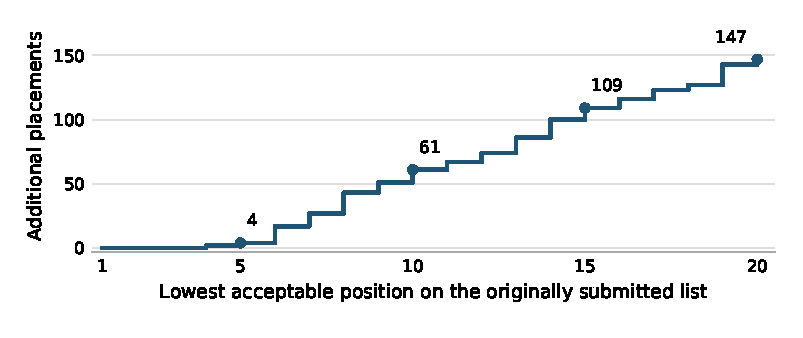
\includegraphics[width=.78\linewidth]{figures/referral-rank.pdf}
\caption{How far down their original lists would applicants have to go? Each point is the maximum number of additional placements compatible with retaining all provisional contracts after the rank-informed university model. A rank limit of five admits four new placements; a limit of twenty admits 147. The horizontal axis is a scenario about acceptable options, not observed take-up.}
\Description{An increasing staircase has 4, 61, 109 and 147 additional placements when referrals may reach original ranks 5, 10, 15 and 20.}
\label{fig:referral-rank}\end{figure}

The attainable gain depends on what the original rule already achieved. Starting from each applicant's first five reported programs allowed 7,268 additional placements in 2026. Starting from the rank-blind network allowed 61. In the 2,304 simulated rental markets, coordinated referrals added 9,749 placements against 5,761 when each applicant chose their favorite vacancy independently. Giving lower-income applicants priority among equally large extensions increased their additional placements from 3,059 to 3,155 with the same total. These are counts across ordinary and enriched simulation draws. Appendix~\ref{app:policy-detail} gives the designs separately and shows what breaks when tentative offers are forecast rather than observed.

\paragraph{How much can exposure alone change affordability?}
Even the most favorable allocation in our 240 calibration markets faces a supply limit. At exactly 217 lower-income placements, the lowest attainable first-quartile asking-rent burden is 27.78\%; among assignments stable on the full graph it is 31.21173\%. Appendix~\ref{sec:burden} gives the matching witnesses and threshold bounds. These statements concern those finite rental markets.
\section{Implications and limits}
A shortlist that retains more historical offers can leave fewer feasible assignments for everyone else. The admissions comparisons supply a way to audit this distinction before deployment. Evaluate the coverage of recorded offers, then replay the full cohort against both a naive baseline and a practical alternative. Check agreement with the historical allocation before interpreting the replay. Participants could change what they submit under an actual quota, so these calculations do not estimate a behavioral treatment effect.

Housing services can know a great deal about asking rents and very little about who would actually apply, who would receive an offer, and who would accept it. Our network learns the consequences of a specified model of those decisions. Sharing donors across months and changing listing panels tests transfer across catalogues, conditional on that model. It does not test behavioral accuracy. In particular, including income as a screening feature can reproduce disparities from the assumed listing rule. A change in the number of stable placements alone says little about housing quality, search costs or realized leases.

A service that already issues tentative offers could record the pre-update lists and offers, apply the priority-blind protection rule, and check whether displaced applicants keep a placement when listings or participants leave during the search. Departures are outside our fixed-market guarantee. A service with no tentative offers would instead need a market-level evaluation and a way to observe how both competing groups fare. In either setting, an applicant with no feasible unit remains unmatched however accurately the model ranks listings. Our original motivation was the possibility that brokers steer clients toward partners. No public input here records referrals or commissions. A test of that hypothesis would require linked impression, referral, offer and acceptance records.
\clearpage
\bibliographystyle{ACM-Reference-Format}
\bibliography{paper}
\clearpage
\appendix
\section{Supplementary results on the two design interventions}\label{app:policy-detail}
\paragraph{How expensive is full visible capacity in the rental panels?}
Using the previously trained contextual network, we compared independent top-five lists with the least-cost displays of Theorem~\ref{thm:capacity-frontier}. Take the attainable capacity range from the original top five up to the full feasible graph; an intermediate policy closes a specified fraction of that gap, rounding its target up to an integer. Priorities and realized preferences enter only the evaluation. In ordinary summer markets the full-capacity policy raises placement by 1.41 points ($[1.26,1.56]$) at a cost of 0.10 points of predicted inclusion probability per renter. In winter these changes are $+1.60$ ($[1.40,1.80]$) and $-0.10$. Measured partner recovery among originally placed renters changes by $+0.02$ and $+0.05$ points, with both intervals spanning zero. In the enriched panels predicted mass falls by 0.39 and 0.53 points, measured recovery falls by 0.57 and 0.68 points and placement rises by 4.29 and 5.58 points. The simpler maximum-weight anchor still places 0.40--0.52 points more than the minimum-loss display in every panel at the same visible capacity. Optimizing the coverage objective can leave room for different stable assignments.

\begin{table}[ht]\centering\small
\caption{Renter placement percentages in 2,304 paired test markets. The fractional targets specify how much of the available increase in matching capacity is required. The final two policies both realize the full feasible graph's maximum matching size on their displays. All rows use the same previously fitted model and five-slot budget.}
\label{tab:rental-frontier}\begin{tabular}{@{}lrrrr@{}}\toprule
 & \multicolumn{2}{c}{Ordinary} & \multicolumn{2}{c}{Enriched}\\
 & Summer & Winter & Summer & Winter\\\midrule
Row top five & 51.22 & 52.83 & 65.21 & 65.86\\
Minimum loss, 25\% of gap & 51.64 & 53.31 & 66.47 & 67.51\\
Minimum loss, 50\% of gap & 51.99 & 53.70 & 67.48 & 68.89\\
Minimum loss, 75\% of gap & 52.41 & 54.16 & 68.69 & 70.42\\
Minimum loss, full capacity & 52.63 & 54.43 & 69.50 & 71.44\\
Maximum-weight anchor, full capacity & 53.12 & 54.95 & 69.93 & 71.84\\\bottomrule
\end{tabular}\end{table}

\paragraph{How much of the vacancy stock can applicants reach?}
We applied Theorem~\ref{thm:residualreferral} after the rank-informed offer network's counterfactual allocation of five programs in the 2026 Chilean university cohort. It left 30,866 applicants without a seat and 21,061 seats vacant. Only 160 of these applicants had submitted any eligible program with an unfilled seat. Within that group, 24 shared just 11 reachable seats. This set witnesses the entire deficit of 13. A maximum flow therefore placed 147 additional people while protecting the provisional recipients. Their median new program was fourteenth on their submitted lists. A follow-up that both maximized cardinality and minimized the sum of entrants' reported ranks moved that median to thirteenth. If referrals must appear among an applicant's top five, ten, or fifteen submitted programs, the exact maxima fall to 4, 61, and 109 respectively. Willingness to accept a lower choice was not observed. Of the 147, seven had been unmatched even under full-list DA and three lacked both a full-list placement and an official regular offer. The other gains chiefly repaired losses created by the original shortlist.

Suppose instead each of the 160 applicants added their favorite program with a vacancy. This placed 156 previously unmatched people, displaced 11 tentative recipients and left 15 tentative recipients with a worse assignment, counting placement loss as worst. In contrast, serially reserving seats placed 144 with zero incumbent losses. DA run as a separate submarket among the eligible applicants and vacancies placed 143 with zero losses. We use previously submitted choices there, unlike the inferred additional schools in \citet{lepesure}. The maximum extension places four more than residual-submarket DA; the median new program ranks were fourteen and thirteen respectively. Maximizing the number of new placements need not select entrants' preferred alternatives.

The first-stage rule makes a large difference to what remains. After the first five submitted choices, the same construction added 5,691, 6,641 and 7,268 placements in the 2024, 2025 and 2026 cohorts. After the 2026 rank-blind network it added only 61. A separate optimistic bound allows incumbents to switch to a weakly preferred program while ignoring the stability constraints on their replacements. It allows at most 204 entrants after the informed network and 2,305 after the blind network, compared with 147 and 61 when all original contracts are held in the witness. Computing this bound starts from the incumbent matching and augments along paths retaining every matched applicant and every incumbent's original ordinal floor. Both the attained flow and its minimum cut were checked.

The rule requires the actual provisional assignment. After replacing priorities by noisy forecasts (independent score errors with standard deviations of 10 and 30 PAES points), choosing apparently vacant slots and then clearing with original scores displaced five and four provisional recipients. These are stress tests with artificial score errors. They do not estimate the accuracy of actual admissions forecasts.

\paragraph{Who can benefit from a second recommendation?}
After the contextual top-five rule in the 2,304 simulated NYC markets, reserved referrals produced 9,749 additional placements with no loss of any tentative recipient. Independent favorite-vacancy referrals produced 5,761; residual-market DA gave 8,460. The allocation among new recipients is still a policy decision. Among maximum-size extensions, favoring lower-income renters increased the number of new lower-income placements from 3,059 to 3,155 at the same total. Under this maximum the ordinary summer and winter panels produced only 13 and 51 additional lower-income placements, against 1,451 and 1,705 additional placements overall. In the deliberately enriched panels, the corresponding numbers were 1,431 of 3,127 and 1,660 of 3,466. Lower-income targeting redistributes the gains that the feasible rental graph permits. All figures are simulated renter instances; the two sampling designs describe different populations.

\paragraph{Finite program capacities.}
The omission bound in Theorem~\ref{thm:omission} extends to programs with integer capacities $u_j$ and strict responsive priorities. Let $H$ again be the applicants whose original assignment is omitted from their display, and $K_j,T_j$ their numbers at program $j$ before and after the restriction. Both gross placement losses and gains are bounded by
\[
                         |H|-\sum_j\min\{K_j,T_j\}.
\]
To see this, removing the members of $H$ and their occupied seats leaves a stable assignment of the other applicants under the residual capacity vectors $u-K$ and $u-T$, respectively. Any block in the residual would have blocked the original. These applicants have the same fixed displayed lists in both residual markets; their original surviving assignments on those lists remain stable after restriction. Raising a single program's capacity by one adds at most one newly matched applicant and removes none. One can replace each capacity by copies with the program's priority, rank copies together in a common fixed order, and insert the last copy by program-proposing DA as in Theorem~\ref{thm:occupied-seats}. Matched-set invariance transfers that statement across stable selections. Comparing the two residual stocks through their coordinatewise minimum bounds incumbent losses by $\sum_j(T_j-K_j)_+$ and gains by $\sum_j(K_j-T_j)_+$. All members of $H$ originally held a place, and $|H|-\sum_jT_j$ lose one, giving the two bounds. Crucially, a recommendation exposes a program with all its seats at once. The quota is a count of programs and the overlap term is a count of seats. These assumptions exclude dynamic sibling priorities and type-specific reserve choice functions.

The protection certificate in Theorem~\ref{thm:threat} also has a many-seat implementation. Build a right vertex for \emph{each protected baseline holder}, keeping their program label. A new outside applicant has an edge to a holder if that applicant sees the holder's program and could outrank the holder there. At most the matching number of this graph of persons can lose their placement. If there are no such edges, every protected holder weakly prefers their new applicant-proposing assignment to their baseline program. To prove both statements, clone program $j$ into $u_j$ seats. All agents rank its seats consecutively in a common order, each with the program's priority. Lift any stable assignment by placing its priority-ordered holders in the consecutively preferred seats. A same-program blocking pair is precluded by this ordering and any cross-program blocking pair would have blocked the original assignment. Conversely, any clone-stable matching induces a stable program assignment. Applicants see all seats of a displayed program and have unchanged rankings across programs. Applying the corresponding unit-seat results proves the count and rank claims; applicant-optimality on the cloned market projects to applicant-optimality over programs. With unknown priorities, aggregate the holders at a program into a single vertex of capacity equal to their number. With known strict priorities the potential targets at one program form a suffix of its holder list. A flow network can share suffix arcs rather than duplicating one edge for every possible holder.

% Section fragment; uses amsthm theorem/corollary environments.
\section{Displacement under deferred acceptance}\label{sec:menu}
Fix unit capacities, strict preferences and individually acceptable visible edges. Incumbents' visible lists and listing priorities over incumbents stay fixed. Outsiders' lists can change. Let $I$ be the incumbents, $H$ the outsiders and $S$ the listings. For $V\subseteq S$, let $F(V)$ be the set of applicants matched by DA in the market of $I$ alone with stock $V$. Restrict lists and priorities to the remaining participants. An incumbent's partner can change even when their match status stays fixed.

\begin{theorem}[Competitors' occupied listings]\label{thm:occupied-seats}
Consider any outcome stable on the display graph of all participants. Write $T$ for the listings occupied by $H$. The set of matched incumbents is exactly $F(S\setminus T)$. If $T$ changes to $T'$, at most $|T'\setminus T|$ incumbents lose a match, and at most $|T\setminus T'|$ gain one. Both bounds hold for any subset of the incumbents.
\end{theorem}
\begin{proof}
Delete all outsiders and their occupied listings. The retained assignments are stable in the residual market because a residual blocking pair would already have blocked the original matching. All stable outcomes of the residual market match the same applicants \citep{galesoto,roth1986}. Its DA thus matches precisely the retained applicants. The argument uses consistency of the stable correspondence \citep{sasaki}. Some remaining applicants can change partners on recomputation.

Run listing-proposing DA on $V$ and retain every proposer's next-choice pointer. Delay a new listing's entry until this run finishes, then let it propose. Each previously held applicant can only trade up among offers and stays matched. The single free proposer continues until a listing exhausts its list or an unmatched applicant holds an offer. Thus adding one listing expands the matched applicant set by zero or one. Matched-set invariance transfers the result to applicant-proposing DA. For two stocks $V,V'$, both $F(V)$ and $F(V')$ contain $F(V\cap V')$. Adding the listings in $V\setminus V'$ one at a time bounds $|F(V)\setminus F(V')|$ by $|V\setminus V'|$. Interchanging $V,V'$ gives the gain bound. Substitute $V=S\setminus T$ and $V'=S\setminus T'$.
\end{proof}

Theorem~\ref{thm:occupied-seats} conditions on the listings outsiders obtain. Anticipating that set can still require solving the counterfactual market. For one outsider $h$, we can identify the affected incumbent before choosing the shortlist. For each listing $s$, let $\ell(s)$ be the sole member of $F(S)\setminus F(S\setminus\{s\})$ or a null label $0$ when this set is empty. Set $\ell(\bot)=0$. The menu $A_h$ consists of listings that give $h$ a match when $h$ lists them alone and the other lists stay fixed.

\begin{corollary}[A menu with displacement labels]\label{cor:displacement}
For a displayed subset $L$ of $h$'s $d$ feasible options, let $w(L)$ be the true favorite in $L\cap A_h$, or $\bot$ if this intersection is empty. Applicant-proposing DA matches $h$ to $w(L)$. Relative to the market without $h$, the missing incumbent is exactly $\ell(w(L))$ if that label is nonzero. For $G\subseteq I$, the change in its number of matched members under $L\to L'$ is
\[
 \mathbf1\{\ell(w(L))\in G\}-\mathbf1\{\ell(w(L'))\in G\}.
\]
\end{corollary}
\begin{proof}
If $h$ receives $s\ne\bot$ under $L$, restricting $h$ to $\{s\}$ preserves this matching's stability. Matched-set invariance implies $h$ is matched under the singleton report and must receive $s$, as in \citep{papai}. Every $j\in L\cap A_h$ is attainable by reporting $j$ alone. If $h$ preferred $j$ to the current partner, or were unmatched despite such an option, that deviation would improve on truthful DA for the preference ordering restricted to $L$, contrary to applicant strategyproofness \citep{roth82}. This is the DA menu principle \citep{menus}. With one outsider the occupied set is empty or consists of their assigned listing. Apply Theorem~\ref{thm:occupied-seats} and take the difference of group counts.
\end{proof}

The listing that accepts $h$ can displace an incumbent who had occupied a different listing. The same identity labels serve every subsequent choice of protected group.

Appendix~\ref{app:menus} derives the exact distribution under uniform quota sampling and the space needed to encode these labels.

\subsection{From one edited list to an entire rollout}
Let $G$ be the group whose lists stay fixed and $H$ the set of editors. For $D\subseteq H$ let $f(D)$ be the number matched in $G$ if exactly the editors in $D$ receive the new list. Begin with a specified baseline realization of everyone's lists. Write $\delta_i=f(\{i\})-f(\varnothing)$ for the effect of changing $i$ alone. The labels in Corollary~\ref{cor:displacement} calculate $\delta_i$ exactly. Now give each editor the new list independently with probability $p$. If $D_p$ denotes the edited set, let $\Phi(p)=\mathbb{E}[f(D_p)]$.

\begin{proposition}[The local rollout effect]\label{prop:rollout}
The initial derivative is $\Phi'(0)=\sum_{i\in H}\delta_i$. Even with common listing priorities and one recommendation per applicant, $\Phi'(0)<0$ and $\Phi(1)>\Phi(0)$ can both hold. The discrepancy between the full change and the derivative can grow linearly with the number of editors.
\end{proposition}
\begin{proof}
Expand $\Phi(p)=\sum_{D\subseteq H}f(D)p^{|D|}(1-p)^{|H|-|D|}$. The constant and singleton terms give the derivative at zero, counting the baseline $-|H|f(\varnothing)$ once. For a family of examples take listings $x_1,\ldots,x_m,z$ with one fixed applicant who sees each listing only. At each $x_j$, two editors outrank the fixed applicant and initially see only $x_j$. Each editor's new list consists of $z$. All listings share a strict ordering with editors first. For $m\ge 2$ an isolated move leaves a competitor at $x_j$ and takes $z$, so every $\delta_i=-1$. If all $2m$ move, the original $m$ listings are available and the fixed applicant at $z$ loses their place. The full change is $m-1$, while the derivative is $-2m$. More generally, each $x_j$ is available with probability $p^2$ and $z$ with probability $(1-p)^{2m}$, so $\Phi(p)=mp^2+(1-p)^{2m}$.
\end{proof}

The result extends to any fixed quota $k$. Add $k$ dummy applicants and $k$ dummy listings. Each dummy applicant ranks a distinct dummy listing first and sees all $k$ dummies. Give every dummy priority over every original applicant at dummy listings; dummy applicants accept only dummy listings. Fill each original list with $k-1$ dummies ranked below its original option. All dummy listings are permanently occupied, preserving the original outcome under every intervention. For any specified order of switching, successive marginal changes telescope to $f(H)-f(\varnothing)$. Computing every marginal at the same baseline discards those interactions. In particular, for a population with a negative initial derivative and positive endpoint change, continuity ensures a sign reversal somewhere along $0<p\le1$.

For quota one the deviation of the joint effect from the sum of the individual effects has sharp bounds (Appendix~\ref{app:menus}).

\section{Protecting tentative offers when recommendations change}\label{app:protect-detail}
A housing service may already know who holds a tentative offer. Can it still use
a learned score to choose other applicants' lists while protecting those offers?
Here protection means keeping a placement; the unit or its rent can change.
Let $M_0$ be stable on the original display. Keep the visible options and
relative preferences of every member of $I$ fixed, and write $H$ for everyone
else. Listing priorities over incumbents are fixed. Let $Q$ be the units
assigned to $I$ in $M_0$, and write $i(j)=M_0^{-1}(j)$ for their holders.
For proposed lists of $H$, draw an edge $hj$ when $j\in Q$, $j$ is displayed
to $h$, and $j$ could prioritize $h$ over $i(j)$ under the information available
to the platform. If priorities are unknown, keep every displayed edge into $Q$.
Write $C$ for this bipartite graph and $\nu(C)$ for its maximum matching size.

\begin{theorem}[A prospective bound on displaced renters]\label{thm:threat}
In every stable outcome on the proposed display, at most $\nu(C)$ previously
matched members of $I$ become unmatched. The bound is attained for every
nonnegative integer value, even at quota one and with a common priority. More
strongly, every bipartite threat graph admits an instance attaining its matching number.
\end{theorem}
\begin{proof}
Write $M_1$ for the new matching. Start at a previously matched incumbent $i$
who is now unmatched. They prefer their old unit $j=M_0(i)$ to their new outcome.
By stability at $M_1$, $j$ has a new holder ranked above $i$. If the holder is
an outsider $h$, we reach a selected edge of $C$. Otherwise the holder $i'$
is an incumbent. The pair $i'j$ was visible before the switch, with $j$ ranking
$i'$ above $i$. Stability at $M_0$ forces $i'$ to have had a partner strictly
preferred to $j$. Continue at $i'$. These walks follow alternating edges in
the symmetric difference of two matchings, whose components are paths and
cycles. The start vertex has degree one, so its component is a path. The walk
can stop only at an outsider. Distinct starting losers give distinct terminal
listings and distinct terminal outsiders: each path is traced from its unmatched
incumbent end to its first outsider, and every noninitial step has a unique
predecessor. Thus the terminal edges form a matching in $C$. For equality take
disjoint copies of one incumbent whose only unit is $j$ and one higher-priority
outsider who switches from a private fallback to $j$.

For sharpness conditional on the graph, give each $j\in Q$ a dedicated incumbent
who accepts only $j$. Choose a maximum matching of $C$. In a common priority put
its matched outsiders first, then all other outsiders, then all incumbents.
Initially every outsider sees only private fallback listings; every incumbent
holds their sole unit. On the new display each outsider sees all its neighbors in
$C$. Matched outsiders rank their respective assigned neighbors first. They take
these distinct listings in priority order. Any unmatched outsider has only
matched neighbors, by maximality, and displaces no additional incumbent.
Private fillers ranked below all neighbors ensure both displays give each
outsider exactly $k$ slots for any $k\ge\max\{1,\Delta_H(C)\}$.
\end{proof}

This is a gross-loss guarantee: it counts an original recipient who loses
their placement even if someone else from the same group gains one. It needs
the observed baseline offers, a stable baseline under the specified display
rule, and unchanged incumbent lists, preferences and within-incumbent priorities.
The priority-blind version treats all higher-priority completions as possible. Computing its graph also needs the feasible choices of each outsider;
it uses neither post-change assignments nor outsiders' rankings. For a single
deployment without baseline offers, the bound cannot be evaluated as stated.
A display can have $\nu(C)>0$ and retain everyone, for example if a threatened
incumbent has an uncontested second choice.

\begin{corollary}[A retained offer as a rank floor]\label{cor:guard-rank}
If $C$ has no edges and the new market uses applicant-proposing DA,
every originally matched member of $I$ receives a unit they weakly
prefer to their original assignment.
\end{corollary}
\begin{proof}
Run DA with one proposal at a time. Suppose some incumbent is rejected or
displaced by their own original unit, and take the first such rejection.
Let $i$ be that incumbent and $j=M_0(i)$ the unit. Unit $j$ holds an
applicant ranked above $i$. An outsider in that position would give a
threat edge. An incumbent $i'$ in that position proposed to $j$. Because
$i'j$ was visible originally and $j$ ranks $i'$ above $i$, original stability
requires $i'$ to have held a unit strictly preferred to $j$. To have proposed
to $j$, $i'$ must already have been rejected by that original unit, contrary
to the choice of the first rejection. Every incumbent's original unit remains
visible. An incumbent ending at a worse option would have received such a
rejection.
\end{proof}
Applicant-proposing DA matters for the rank floor. For two incumbents with
opposite top choices, let each unit rank its other applicant first. The
applicant-optimal and unit-optimal matchings are both stable. Switching
between them can make both incumbents worse off with no outsiders at all.
The rank floor still permits a higher rent for a more-preferred unit.

A budget of one already permits arbitrarily many rank losses with no one
becoming unmatched. For $n$ incumbents, applicant $i$ ranks $s_i$ over
$s_{i+1}$ for $1\le i\le n$. One outsider switches from their private
fallback $z$ to $s_1$. The common priority puts the outsider first, then
incumbents in increasing order. Initially all incumbents get their first
choice; on rollout each gets their second. Only the outsider's edge to $s_1$
is a threat. Giving the outsider the same private, last-ranked filler on both
displays preserves a universal quota of two.

With known priorities, the first-rejection argument also locates possible rank losses when $C$ has edges. Start at the holders of threatened units. From baseline holder $a$ draw an arrow to holder $b$ if $a$ can see $M_0(b)$ and outranks $b$ there. Every rejected holder is reachable from a start: a rejection by an outsider starts a path, and a rejection by another fixed applicant extends a path from that applicant's earlier rejection. Induction over the rejection times proves the claim. It explains why regions of the market can stay protected even if the overall budget is positive.

\paragraph{Choosing a display with a loss budget.}
Let $q_h=\min\{k,d_h\}$, and let $w_{hj}$ be any score estimated before the
switch. On all feasible outsider edges use binary display indicators $x_{hj}$.
On the full set $C_*$ of possible threats use binary cover indicators
$a_h,b_j$ at their endpoints. Solve
\[
 \max \sum_{hj}w_{hj}x_{hj}
 \quad\text{subject to}\quad
 \sum_j x_{hj}=q_h,\qquad
 x_{hj}\le a_h+b_j\ (hj\in C_*),\qquad
 \sum_h a_h+\sum_{j\in Q}b_j\le B .
\]
By K\H{o}nig's bipartite matching theorem, a proposed display admits such
a cover exactly when its certificate $\nu(C)$ is at most $B$. At zero budget
each outsider receives their $q_h$ highest-scoring feasible options outside
the threat edges; feasibility requires and suffices that every row has $q_h$
such choices. If no certified slate exists, retaining the entire baseline
display preserves quotas and placements even when the baseline graph itself
has positive certificate. The following refinement can let other applicants switch.

\paragraph{Preserving every quota when a row has too few safe options.}
Start with $J=I$. Hold every $J$ row at its original ordered display and
protect the baseline units of all matched members of $J$. For each $h\notin J$
count its feasible nonthreat edges under this enlarged fixed set. If any
applicant cannot fill their quota, add all such applicants to $J$, retaining
their original displays. Repeat until each remaining applicant can fill their
quota, then display their top-scoring nonthreat options. The procedure stops
within $|H|$ nonempty rounds and preserves every quota. Theorem~\ref{thm:threat}
at the final $J$ gives zero losses among the initially matched members of $I$. Corollary~\ref{cor:guard-rank} also protects their original ranks under applicant-proposing DA.
For closure, fix in advance which listing priority comparisons are known; if more applicants are frozen, the information used for a given comparison stays fixed. The final $J$ is contained in any superset of $I$ that would admit complete
quota-respecting lists and a zero-threat certificate for all its members.
Indeed, given $J\subseteq J'$, a row deficient at $J$ must belong to any such
$J'$: as long as this row remains outside, enlarging $J$ only removes safe
edges. Induction proves the claim. The minimum freeze set is relative to this
specific certificate; another stable display can sometimes protect all renters
with fewer freezes. If every applicant is frozen, the original display returns.

\paragraph{The cost of a positive loss budget.}
Deciding whether a display can reach score $W$ subject to a certificate budget
$B$ is NP-complete even at quota one, with binary scores, at most three feasible
listings per outsider and a common strict priority. Reduce from Vertex Cover.
Make a unit for each graph vertex, held by a dedicated incumbent whose only
option is that unit. Introduce an outsider for each graph edge, with its two
endpoint units scoring one and a private fallback scoring zero. Initially each
outsider sees their fallback, and every incumbent holds their own unit. Give
every outsider higher priority than every incumbent. Set $W$ equal to the
number of edges. Every outsider must now nominate one endpoint. The selected
threat graph has outsider-degree one, so its matching number equals the number
of distinct nominated endpoints. These form a vertex cover. Conversely any
vertex cover permits each outsider to nominate one of its endpoints. Both
displays have one entry per applicant. Verifying the score, quotas and
matching number takes polynomial time. Thus finding the best score under
a variable loss budget can require combinatorial optimization, while checking
the certificate for a given display is efficient.

\section{Additional experiments and replication}
\subsection{Choosing how often to deploy a policy}\label{sec:risk}
Suppose a service can try a new rule in a whole market or keep the current rule throughout that market. Let $L$ be the event that at least one lower-income renter who was placed under uniform exposure loses their placement when only higher-income shortlists switch. A market where two gain and one loses still counts as a loss event. A platform would need both potential outcomes to label $L$; we can compute the pair in this simulator. This risk differs from the probability that a randomly chosen renter loses a placement.

Our calibration uses the finite-sample risk-control principle of \citet{ltt,riskrec}. Let $Z_{bj}\in[0,1]$ be the weighted fraction of the twelve borough-month markets in independent seed block $b$ where policy $j$ incurs $L$. The weights describe a draw of one market from the target mixture. For $n$ calibration blocks and $m$ prespecified comparisons, let $U_j$ be the largest $u\in[\bar Z_j,1]$ satisfying
\[
 n\,\mathrm{kl}(\bar Z_j,u)\le\log(m/\alpha),
 \quad
 \mathrm{kl}(x,u)=x\log(x/u)+(1-x)\log((1-x)/(1-u)).
\]
Use the usual endpoint limits. With probability at least $1-\alpha$, the true market risks are at most $U_j$ for all $j$. To see this, for $0\le Z\le1$ convexity bounds $\mathbb E e^{tZ}$ by $1-\mu+\mu e^t$ where $\mu=\mathbb E Z$. Applying the lower-tail Chernoff bound to independent blocks gives $\Pr(\bar Z\le x)\le e^{-n\mathrm{kl}(x,\mu)}$ for $x<\mu$. Inversion and a union bound give the claim. No independence between policies or among the twelve markets in a block is needed.

For a target $\tau>0$, deploy in a fraction $q_j=\min(1,\tau/U_j)$ of markets using one coin independent of the market (set $q_j=1$ when $U_j=0$). On the joint coverage event its risk is $q_j\mathbb E Z_{bj}\le\tau$, including after a choice among the calibrated policies. Using an independent coin per renter would instead move to a different point on the interference curve of Proposition~\ref{prop:rollout}. The guarantee is over repeated draws from the same simulator and a service willing to keep uniform exposure in the other markets. It offers no individual right to retain an offer and no guarantee under temporal shift.

We set $\alpha=0.05$ and calibrate twelve bounds, one per combination of design, score (transparent, pointwise, contextual) and decoder (row top five or anchor). We use 32 separate summer calibration blocks (768 markets) reserved before fitting. At $\tau=0.05$, for the contextual top-five rule the ordinary calibration event rate is 16.96\%, with a simultaneous upper bound of 44.53\%. This admits rollout to 11.23\% of markets. In the enriched design the calibration rate is 81.76\%, the upper bound is 96.63\%, and the permitted fraction is 5.17\%. On the independent summer test these choices give expected loss-event frequencies of 1.95\% and 4.26\%, integrating over the deployment coin analytically. In winter they give 2.64\% and 4.29\%. The small number of calibration blocks and the simultaneous guarantee make the limits conservative. Full results at 1\%, 5\% and 10\% are archived. The deterministic rule in Theorem~\ref{thm:threat} can make finer changes because it observes the provisional allocation.

\subsection{A two-sided recommendation benchmark}
\label{app:su-replication}
In the interview model of Su, Bayoumi and Joachims~\cite{rankings}, applicants may receive several invitations. Can we reproduce the congestion result before adapting their approach to rentals? We ran the authors' released solver and evaluation code with 30 applicants, 20 employers, crowding $0.5$ and inverse-rank attention. Each of ten market seeds (621--630) was simulated 10,000 times per policy. Naive, reciprocal and welfare ranking produced 18.41, 20.86 and 22.77 expected interviews, respectively. The release reports 18.7, 21.2 and 23.2. The authors give a default seed but do not list their full ten-seed set. We corrected an undefined variable used to save the final file after optimization.

We also evaluated expected interviews directly. If applicant $i$ applies to listing $j$ with probability $a_{ij}$, their expected examination probability given application is
\[
  \int_0^1 \prod_{h\succ_j i}(1-a_{hj}+a_{hj}t)\,dt.
\]
Indeed, if $N$ higher-priority applicants apply, $1/(1+N)=\int_0^1 t^N\,dt$. Independence across applicants gives the product. Multiplication by $a_{ij}$ and reciprocal-side relevance and summation over pairs gives expected interviews. With 100 employers and 150 applicants, the release-order welfare and reciprocal methods yielded 199.12 and 201.05 at zero crowding, 152.30 and 129.97 at half crowding and 117.37 and 91.33 at full crowding. The released optimizer iterates the inverse of the permutation of applicants in decreasing employer relevance. The equations specify the decreasing-relevance permutation itself. With this second order the corresponding welfare estimates were 203.52, 154.09 and 117.37. Both variants were evaluated using decreasing employer relevance, as in the authors' evaluator.

On the authors' 925-participant conference-networking matrix of imputed relevance, we removed self-pairs and reranked the first 100 reciprocal suggestions as specified in the paper. We obtained 603.0 and 764.1 expected successful replies for naive and reciprocal ranking, close to the published 604.0 and 763.9. Our equation-order welfare ranking reached 862.8, compared with the published 824.1. The policy ordering replicated. The difference in the optimized value remains unexplained. These outcomes are model expectations conditional on imputed relevance.

For the rental adaptation we used observable-score midranks within each renter's feasible listings and within each listing's eligible renters as proxies $f_{ij}$ and $g_{ij}$ for bilateral relevance. Each midrank is the average tied rank minus one half, divided by its comparison-set size. We used the paper's descending priority order. If $x_{ij}$ denotes display probability, application probability in the surrogate is $a_{ij}=f_{ij}x_{ij}$. We optimized its inverse-rank Jensen bound
\[
  \sum_{ij} \frac{g_{ij}a_{ij}}{1+\sum_{h\succ_j i}a_{hj}}
\]
over the row-wise convex hull of feasible top-five menus, initialized uniformly. Each of 50 Frank--Wolfe steps has size $0.2$. The linear oracle sorts the exposure gradient in each row. We displayed the five largest feasible final exposures (or all if fewer than five), resolving ties by independent market-keyed permutations. Deferred acceptance then ran on the resulting graph with unit capacities and the same latent preferences used for every housing comparison. The rank probabilities and the hard display quota are modeling choices. Expected replies and realized one-to-one allocations can favor different menus.

\section{Learning checks and sensitivity analyses}\label{app:ai}
We used width 32, SiLU activations, 28 epochs of AdamW (step size 0.002, weight decay 0.0001), batches of 32 markets and gradient clipping at norm 3. Feasible training edges determine feature means and scales. We fit each architecture at seeds 8101--8103, selected the epoch of minimum validation cross-entropy separately for each seed, and averaged the three predictive distributions. The contextual network sends means and log degrees of adjacent edge sets through two residual updates. The pointwise version retains the edge encoder and the outside head's row pooling. The additional capacity control is described below. Training, model selection, independent rollout calibration, summer testing and winter testing used five disjoint seed ranges. Donor households can recur in all five. The listing panel is shared between summer splits. The winter catalogue removed identifiable summer duplicates before drawing. The code tracks input hashes, model checkpoints and exactly which studies used each panel. The complete synthetic market is known for computing the training label and evaluating policies. Only observable features and feasibility enter a fitted model at inference.
\begin{table}[t]\centering\small
\caption{Placement under five-listing recommendations to all applicants (percent). Each column uses 576 paired markets. The first five rows choose a separate shortlist for each renter or use the two-sided surrogate. The last three reserve one slot using a market-wide assignment.}
\label{tab:ai}
\begin{tabular}{@{}lrrrr@{}}\toprule
 & \multicolumn{2}{c}{Summer} & \multicolumn{2}{c}{Winter} \\
\cmidrule(lr){2-3}\cmidrule(l){4-5}
Policy & Ordinary & Enriched & Ordinary & Enriched \\\midrule
Uniform & 54.30 & 66.39 & 56.18 & 68.24 \\
Transparent & 30.79 & 36.10 & 31.37 & 35.11 \\
Two-sided surrogate & 51.47 & 61.60 & 53.74 & 63.02 \\
Pointwise & 45.12 & 59.13 & 46.56 & 59.71 \\
Contextual & 51.22 & 65.21 & 52.83 & 65.86 \\
\midrule
Transparent + anchor & 51.63 & 68.99 & 53.45 & 72.07 \\
Pointwise + anchor & 51.18 & 68.70 & 53.13 & 70.98 \\
Contextual + anchor & 53.12 & 69.93 & 54.95 & 71.84 \\
\bottomrule\end{tabular}\end{table}

\paragraph{Is the gain due to seeing competitors?}
The basic pointwise ablation removes layers as well as information. Following the original comparison, we trained an additional own-row model, keeping the contextual architecture's 11,906 trainable parameters and three initialization seeds. In place of every column message it receives the focal edge's embedding and the renter's own row degree. It can compare all options for one renter. It sees no other renter. The contextual model raised total placement relative to this equal-size comparator by 1.91 points (95\% paired interval $[1.64,2.17]$) in summer ordinary, 2.08 $[1.82,2.35]$ in winter ordinary, 2.82 $[2.53,3.11]$ in summer enriched and 2.67 $[2.35,2.99]$ in winter enriched. Partner recovery improved by 1.30, 1.42, 1.88 and 1.94 points, respectively. This control reduces the share of the original pointwise comparison that can be attributed to competitor information.

\paragraph{Repeated simulation under the training law.}
We drew 128 independent sets of hidden preference shocks for each of 384 test markets (the first eight blocks in each season). Each draw keeps eligibility and observable utility fixed. We solved full-exposure DA, estimated the probability of each partner by its frequency, and selected five feasible units per renter. This benchmark has the simulator's shock law at prediction time. The realized test ranks never enter its predictions. All 49,152 independent conditional solutions were checked for visible blockers and feasibility. The comparison uses a common finite panel and does not multiply the number of independent boroughs or household draws by 128. A subsequent precision check increases the conditional sample, as reported below.

At 128 draws the contextual model recovered more partners than conditional simulation in every panel. We therefore increased the simulation budget on the same panels, without changing features, policy or tie resolution. An independent stream with 2,048 draws per panel market gave 786,432 additional verified stable assignments. At this precision the recovery gap narrowed to at most 0.63 points (Table~\ref{tab:mc}). These are paired point estimates on eight blocks per season. The simulation comparator knows the stipulated preference law; this calculation cannot establish how much either method knows about actual renters.
\begin{table}[ht]\centering\small
\caption{Full-market partner recovery (percent) on the same 384 markets. The first two simulation columns share draws with the 128-draw run, while 512 and 2,048 use a separate nested stream. The neural model scores one observed market without drawing latent preferences.}
\label{tab:mc}
\begin{tabular}{@{}lrrrrrr@{}}\toprule
Market & 16 draws & 64 & 128 & 512 & 2,048 & Contextual\\\midrule
Summer ordinary & 33.49 & 35.04 & 37.88 & 39.83 & 40.64 & 40.51\\
Summer enriched & 27.39 & 30.76 & 32.32 & 33.85 & 34.60 & 35.23\\
Winter ordinary & 31.06 & 33.28 & 35.87 & 38.06 & 38.95 & 38.94\\
Winter enriched & 26.63 & 29.59 & 31.34 & 32.83 & 34.03 & 34.04\\\bottomrule
\end{tabular}\end{table}

\paragraph{Numerical reproducibility.}
The archive contains the trained weights, full training traces and frozen scores used to generate the reported lists. A CPU replay from the same weights on 1,152 summer test markets changed 434 of 73,728 contextual top-five lists and 130 binary placement outcomes. For the anchored version, 2,445 lists and 650 placement statuses changed. Both CPU policies placed ten more renters in aggregate than their corresponding GPU runs. Near-ties can move identifiable simulated renters even when aggregate placement is similar. The theoretical guarantee applies to either realized display once the protection rule is applied.

\subsection{Which results rely on landlord income screening?}
\label{app:income-stress}
The screening coefficient is a modeling assumption. In eight seed blocks per season we held the menus, renter rankings, features and trained networks fixed. We drew one independent standard-normal shock per pair. Landlord priorities were the shock plus either zero or $2.5$ times the capped income-to-annual-rent ratio. Changing this coefficient only at allocation time tests how a fixed policy behaves when the landlord rule differs from the training model. We paired both runs on the same shocks in all 384 markets. Our subgroup rate divides the geographically weighted number matched by the weighted number of renters in the group within each block, including renters with no listings. Intervals are marginal 95\% Student intervals over eight paired simulation blocks per season.

\begin{table}[t]
\centering\small
\caption{Lower-income match rate when only higher-income renters receive the contextual top-five policy. Uniform and context give percentages. The final column gives the percentage-point difference versus uniform menus and its paired interval.}
\label{tab:screen-stress}
\begin{tabular}{llrrrr}
\toprule
Supply & Period & Coefficient & Uniform & Context & Difference [95\% interval]\\
\midrule
Ordinary & Summer & 0 & 5.40 & 4.95 & $-0.44$ [$-0.90$, $0.02$]\\
 & & 2.5 & 3.03 & 2.49 & $-0.54$ [$-0.71$, $-0.37$]\\
 & Winter & 0 & 7.28 & 6.70 & $-0.58$ [$-1.18$, $0.02$]\\
 & & 2.5 & 4.43 & 3.69 & $-0.74$ [$-1.20$, $-0.28$]\\
Enriched & Summer & 0 & 51.20 & 55.23 & 4.04 [2.49, 5.58]\\
 & & 2.5 & 36.96 & 44.69 & 7.72 [5.46, 9.99]\\
 & Winter & 0 & 54.30 & 58.46 & 4.16 [2.79, 5.53]\\
 & & 2.5 & 40.01 & 47.48 & 7.47 [5.21, 9.73]\\
\bottomrule
\end{tabular}
\end{table}

In the enriched markets the positive spillover persisted when listings ignored income. Its size fell by 3.69 points in summer [1.75, 5.63] and 3.31 in winter [1.48, 5.14]. Absolute match rates for lower-income renters rose without income screening under both menus (Table~\ref{tab:screen-stress}). With all renters receiving the coordinated contextual menu, its total placement gains over uniform in enriched markets also persisted at coefficient zero, at 1.00 [0.59, 1.40] and 2.12 [0.90, 3.34] points respectively. For ordinary supply that same policy lowered total placement by 3.41 [2.83, 3.98] and 3.20 [2.27, 4.13] points. Marginal intervals and raw rates for every policy and both groups are supplied with the artifact.


\section{Data and replay for observed-preference markets}
\subsection{Regular university admissions in Chile}\label{app:paes}
The public PAES applications list each student's program choices in order, their program-specific weighted score and their official status. Our capacity equals the sum of first- and second-semester regular seats and announced overbooking seats. We keep regular applications coded selected, waitlisted or passed over following a higher selection (24, 25, 26). We rank by weighted score and break score ties by a fixed seeded lottery. In a check that omits all test-year status codes when selecting candidate edges, keeping valid nonduplicate reported programs with a strictly positive score gives exactly the same applicant--program pairs, order and scores in 2026. We never distinguish selected from waitlisted when producing a 2026 display. Program-specific selection rank and individual identifiers do not enter the predictor. The public input omits five applicants in 2026 for confidentiality. A recorded offer is an invitation to enroll. Subsequent enrollment and waitlist movements are different outcomes.

The 2024 and 2025 cohorts have 188,707 and 189,982 regular applicants. For the 2025 model, we use each program's previous minimum regular offer score and reported demand per seat from 2024. Missing program cutoffs receive the median available cutoff; missing congestion receives the median across prior programs. Ridge logistic regression with a fixed feature basis uses log submitted rank, log list length, score, cutoff distance, capacity and interactions. Its label is the matched edge under full-list applicant-proposing DA (zero for every other edge). The year-ahead run applies the same coefficients to 2026 features using 2025 historical summaries. A second control keeps programs where the weighted score clears last year's program cutoff, in applicant rank order, then fills any remaining slots from the other programs. All displayed programs are proposed to in original preference order. These rules could be evaluated after applications are drafted. They are not search tools for programs the student never considered.

\begin{table}[ht]\centering\small
\caption{Chilean university menus. The first numeric column measures recovery among 156,248 recorded regular recipients. The second uses 158,697 full-list DA recipients. The third uses all 189,399 applicants. The last two columns show the placement change against uniform for caps of one and ten choices. Uniform coverage is analytic; placement averages 64 draws.}
\label{tab:paes}\begin{tabular}{@{}lrrrrr@{}}\toprule
 &\multicolumn{3}{c}{Quota five, percent}&\multicolumn{2}{c}{Placement change (pp)}\\
\cmidrule(lr){2-4}\cmidrule(l){5-6}
Rule & Recorded offer & DA partner & DA placed & Quota one & Quota ten\\\midrule
Uniform & 74.22 & 73.83 & 82.27 & --- & ---\\
First reported choices & 91.00 & 89.98 & 79.20 & $-9.68$ & $-0.87$\\
Historical cutoff & 95.90 & 96.35 & 83.74 & $+9.42$ & $+0.17$\\
Fitted classifier & 98.05 & 97.64 & 83.19 & $+8.16$ & $+0.05$\\\bottomrule
\end{tabular}\end{table}

At quota three the classifier placed 155,593 students, versus 157,932 under the cutoff rule and 150,804 on average under uniform. At five, 96,310 applicants had enough options for pruning to bind. The standard error of the mean uniform placement count was 7.8 applicants (0.0041 percentage points). The deterministic policies have no corresponding display-sampling error. Removing overbooking reduces full-list agreement with recorded offers to 105,097 of 156,248 recipients (67.26\%). The fitted rule still places more applicants than uniform and fewer than the historical-cutoff control at five choices (139,039 versus 138,448 and 139,799). Two independently written DA algorithms, sequential and simultaneous, gave identical full-market assignments. Every evaluated display passed capacity and no-blocking-pair checks. A max-flow calculation verified each displayed capacity with an equal-valued cut.
\paragraph{Prediction from recorded offers.}
As a follow-up we fitted equal-size, row-permutation-equivariant networks to the actual 2025 regular offer or the outside option. Both networks receive program selection score, score relative to the previous cutoff, previous demand per seat, current capacity, and a missing-history indicator. One also receives reported preference rank. Options are permuted independently in every applicant row, lifting any dependence on column position. Each setting uses three H200 fits, a fixed 12 epochs and average predicted probabilities. There are no 2026 labels in the inference files. Both models are evaluated at the same four quotas in the same 2026 cohort as the primary analysis. The outcome-blind construction found the same 1,328,381 eligible pairs.

With five programs, the rank-blind model retained 144,401 of the recorded regular offers (92.42\%) and placed 158,800 applicants. Giving the same architecture the submitted rank retained 155,657 offers (99.62\%) and placed 158,533. This is a gain of 11,256 covered historical offers and a net loss of 267 counterfactual placements. Relative to full-list DA, the rank-informed model caused fewer members of the original placed set to lose a place (364 versus 1,045). It also placed far fewer previously unmatched people (200 versus 1,148). The additional 681 retained recipients and 948 fewer entrants sum to the 267-placement loss. This distinction is important when the service both predicts historical offers and evaluates policy performance on previous recipients.

\subsection{Validating against observed university registrations}\label{app:enroll}
We used the ministry's separate PAES registration file, with applicant pseudonyms used only to link records locally \citep{paes}. It contains 146,873 unique students for 2026. Of these, 10,122 fall outside our regular applicant cohort. Of the 189,399 regular applicants, 136,751 have a link and 52,648 have no registration record in this release. The coverage denominator is the 136,751 linked applicants, including 5,271 whose destination is absent from the retained regular graph. The file covers several admission routes. No record here need not mean that the applicant did not attend any institution.

\begin{table}[ht]\centering\small
\caption{Five-program lists produced by the two offer-trained networks. Historical regular offer describes the program in which a registered applicant was initially invited to enroll. Gains and losses count individual enrolled destinations added or removed by supplying the network with submitted rank.}
\label{tab:enroll}\begin{tabular}{@{}lrrrrr@{}}\toprule
Historical regular offer & Students & Blind coverage & Informed coverage & Gained & Lost\\\midrule
Registered there & 116,638 & 107,773 & 116,284 & 8,580 & 69\\
Registered elsewhere & 10,264 & 5,758 & 7,063 & 1,446 & 141\\
No initial regular offer & 9,849 & 5,367 & 6,321 & 976 & 22\\\midrule
All linked applicants & 136,751 & 118,898 & 129,668 & 11,002 & 232\\\bottomrule
\end{tabular}\end{table}
\paragraph{Changing what the network learns.}
The offer comparison prompted a paired follow-up on the same cohort. We replaced only the target in the 2025 training data, retaining each applicant's enrolled program when it appeared on the regular applications, or the outside class otherwise. This changes 45,450 of 189,982 training labels. We used the same row masks, features, shuffling, two architectures, seeds, optimizer, epochs and 2026 test features. The outside class describes missing on-list enrollment and includes registration through other routes. We selected no epoch or scoring rule using the test results.

All six H200 runs completed. With enrollment as the training target, the rank-blind and rank-informed menus covered 119,414 and 130,305 of the 136,751 linked registrations. The informed menus thus covered 10,891 more actual destinations. Replayed DA placed 158,498 and 158,357 applicants, respectively, a loss of 141. The informed model kept 612 more original full-list recipients placed (1,239 versus 627 losses) but brought in 753 fewer previously unmatched applicants (1,040 versus 287 entrants). Training on registrations therefore preserved the within-architecture sign pair on this cohort. It also reveals a distinction between objectives: versus the offer-trained informed model, the enrollment-trained informed model covered 637 more registered destinations, covered 79 fewer initial offers, and placed 176 fewer applicants. The individual-level records and predictions stay out of the shared archive.



\subsection{Chilean school admission reports}\label{app:sae}
The Ministry's A1 files give program vacancies; B1 gives the applicant and grade; C1 records the ordered applications with course-level lottery and priority; D1 records the initial offer, before applicants respond. Program means a course within a school, since specialties and schedules can differ at the same school. The 2019 fit uses 483,070 applicants. Application years 2020 and 2021 contribute 454,415 and 461,223 applicants, including those who received no offer. Individuals can apply in successive years; no individual identifier enters the model. Outside the reported list, preferences are unknown. The exercise randomly or systematically prunes a submitted list. It makes no assumption that families supplied truthful rankings over schools they left off that list.

Both fitted rules are ridge logistic edge models trained on whether the initial 2019 offer equals that program. The rank-blind model uses log capacity and demand, a squared congestion term, coarse priority indicators, list length, grade and a smoothed 2019 program offer rate. The last feature is leave-one-out on the training cohort and fixed on test cohorts. Known priorities include returning, sibling, staff-child and former-student statuses. A protected entitlement remains available at every quota and options ranked below it are dropped. The rank-informed model adds log position, an indicator for the first choice and an interaction between position and congestion. Fitted coefficients, exact features and penalty are archived. We retain the highest-scoring $\min(k,d)$ discretionary options and preserve their submitted order. Uniform draws assign an independent random order to the discretionary options. Priorities and lists used for counterfactual allocation are identical across all arms except for policy pruning.

For allocation the benchmark pools vacancies across seat types, ranks applicants by the published priority tier and then by the realized lottery order at that course. At programs with fewer reported vacancies than secured current-school claims, the pooled capacity is raised just enough to accommodate them (6,582 and 6,815 seats across the two years). Grade cohorts are disjoint under fixed priorities. The actual system uses special reserves and family contingencies \citep{correaschool,saereserve}. Its exact published course or outside option agrees with full-list benchmark DA for 432,783 and 440,582 applicants. Official offers below the retained entitlement or off the retained list count as uncovered (3 and 7). C1 appends a current school even when the family did not request it. Excluding placements at such administrative additions from the placement numerator preserves the directions of both five-choice model comparisons. This is a cross-domain test among reported alternatives. Its predictors, population, capacities and use of preference reports differ from those of the rental study.

\begin{table}[t]\centering\small
\caption{Chilean regular-round school admissions. Coverage measures how often an applicant's reference course appears on the five-choice menu plus protected entitlement among applicants assigned by that reference. Placement is the share of all applicants assigned by pooled-seat DA. Uniform reports the mean of 48 independent menu draws per cohort.}
\label{tab:sae}\begin{tabular}{@{}llrrr@{}}\toprule
Cycle & Menu & Official offer (\%) & Full-list DA offer (\%) & DA placed (\%)\\\midrule
2020 & Uniform & 97.59 & 97.57 & 90.66\\
 & First reported choices & 98.77 & 98.83 & 90.34\\
 & Rank-blind prediction & 99.39 & 99.38 & 90.94\\
 & Rank-informed prediction & 99.71 & 99.73 & 90.82\\\midrule
2021 & Uniform & 97.94 & 97.93 & 91.53\\
 & First reported choices & 99.03 & 99.07 & 91.28\\
 & Rank-blind prediction & 99.46 & 99.44 & 91.77\\
 & Rank-informed prediction & 99.79 & 99.80 & 91.66\\\bottomrule\end{tabular}\end{table}

Only 37,312 and 33,570 applicants have more than five discretionary choices. Their rank-blind placement gains relative to uniform were 4.84 and 4.28 points. The other 417,103 and 427,653 applicants experience placement losses of 0.13 and 0.07 points as competitors' lists change. Both official coverage and overall placement increase for the rank-blind model relative to uniform in all 14 grade cohorts in each year. Standard errors over random menus quantify numerical integration only; the 95\% Monte Carlo half-width on the two aggregate placement contrasts is below 0.003 percentage points. Finite-population counts require no independence assumption across applicants. The second ranker and quotas $k=1,2,3$ were specified before scoring, with the comparison between the two fitted models interpreted after observing the primary result. The archive also gives all grade and designated-priority subgroup counts.

As a follow-up, we held the two learned scores fixed and varied the capacity specification. With unadjusted published vacancies, the five-choice rank-blind placement gains relative to uniform were 0.283 and 0.252 points; relative to rank-blind, rank-informed placement fell 0.117 points in both years. With only ordinary vacancies and the same current-school capacity floor, the corresponding paired differences were $+0.281,-0.122$ and $+0.228,-0.114$ points. Neither sensitivity fully implements the deployed reserve routing. A separately implemented simultaneous-offers DA verified every applicant's final program under full exposure and each deterministic five-choice rule, a total of 3,662,552 person--policy checks. For uniform coverage we also summed the exact inclusion probabilities of each reference edge. The Monte Carlo estimates lay within two Monte Carlo standard errors across the sixteen year, reference and quota comparisons.

\subsection{Confirmation and spillovers in the school cohorts}\label{app:sae-fresh}
We retained the procedures in Appendix~\ref{app:sae}, including every grade, the program-specific realized lottery, entitlement floor and continuity option outside the five discretionary slots. The model uses the 2019 fitted coefficients and 2019 program frequencies in every test cycle. The new regular-round archives supply the same fields used in 2020--21. Application years 2022 and 2023 correspond to admission years 2023 and 2024. The recorded initial course can be compared with menu membership even though the allocation under a changed display is a counterfactual. The sign criterion was specified separately for each year before obtaining these releases. No applicant-level independence or between-year inferential interval is assumed. The two cohorts contain 520,420 and 492,888 officially assigned applicants, respectively. Outside outcomes, including students with no discretionary choice, count toward the placement denominator.

\begin{table}[t]\centering\small
\caption{Previously unexamined school application cycles. Rank-informed minus rank-blind at five discretionary choices. A recorded offer counts as covered if present in the display. The last columns partition the placement change by whether the pupil would receive a place under full-list pooled DA.}
\label{tab:sae-later}
\begin{tabular}{@{}lrrrrr@{}}\toprule
Year & Applicants & $\Delta$ coverage & $\Delta$ placed & $\Delta$ retained & $\Delta$ entrants\\\midrule
2022 & 570,891 & $+1,143$ & $-468$ & $-110$ & $-358$\\
2023 & 536,353 & $+1,350$ & $-517$ & $-117$ & $-400$\\\bottomrule
\end{tabular}\end{table}

\paragraph{Whose list changed?}
The B1 field \textit{prioritario} identifies families with an administrative priority designation. It supplies neither measured household income nor a randomized group assignment. We computed all four combinations of which group's long lists use the rank-informed score. When \emph{only other applicants} switch, every designated pupil has exactly the same menu as before. Among designated pupils in 2022, 127 lost a placement and 67 gained one; in 2023, 125 lost and 60 gained. In both years this is an externality on people who never received the new ranking. Under universal use, the designated group's net placement change per hundred applicants was $-0.050$ and $-0.064$ points, versus $-0.126$ and $-0.148$ among other applicants. Standardizing both groups to the pooled grade, discretionary list-length band and entitlement distribution gives $-0.064$ and $-0.077$ versus $-0.103$ and $-0.126$. All strata for 2022/23 contain both groups. Group composition explains part of the raw gap. These descriptive contrasts do not isolate a causal effect of priority status.

\paragraph{Representing reserved places.}
The primary one-pool replay omits the allocation of earmarked vacancies. As a sensitivity, each program first retains returning pupils, then uses up to its published \textit{vacantes prioritarios} places for remaining designated pupils, allowing any unfilled reserve to revert to the open pool. Each step uses the original coarse priority and realized lottery. This simplified reserve-first rule omits other reserve types, dynamic family links and the ministry's full sequence of assignments. The full-list exact program/outside agreement rises slightly from 95.385\% to 95.414\% in 2022 and from 95.785\% to 95.800\% in 2023. At five choices the ranking switch reduces placements by 469 and 516 under the sensitivity, close to the pooled losses of 468 and 517. Official-offer coverage does not depend on the subsequent allocation rule. The archive gives gross flows, rank changes for those remaining matched, and editing-group decompositions for each of the four years.

\paragraph{Offers families actually accepted.}
As a follow-up we restricted the administrative coverage target to applicants whose parent or guardian explicitly accepted the initial offer, including those who accepted while waiting for a more preferred course. The 2022 and 2023 cohorts have 382,638 and 367,749 such records. Rank-informed menus covered 1,000 and 1,244 more of their accepted initial courses than rank-blind menus. Thus 2,244 of the overall 2,493 net additional covered initial offers belong to explicit acceptances. We did not infer acceptance for nonrespondents or observe what families would have accepted under a shortened menu.

\subsection{Mutually submitted mentoring ranks}
Haas and Hall release the weak preference orders submitted in three annual one-to-one mentoring markets \citep{haashall2019}. We learn from the first two numbered scenarios and evaluate on the third. The third workbook tab contains 29 mentees, 38 mentors and 154 mutually listed pairs; 33 mentors have an eligible pair. All 29 mentees remain in the placement denominator. The source reports 28 mentees in its first summary table and 29 in its subsequent parameter table. Ties are real responses. We independently draw strict refinements within tied tiers and hold the resulting orders fixed across policies. Full exposure is the complete set of mutual reports. The outcome is a counterfactual mentee-proposing DA allocation on this graph. The workbook does not record how participants would respond to different shortlists or supply their realized field assignments.

A regularized multinomial model uses both reported midranks, degrees and competition for first-tier choices. It learns full-report partner probabilities from 4,096 tie refinements of each training cohort. A graph-only model omits reported rank and first-choice information. At inference the learned rules see the weak profile, never the strict evaluation refinement. Thus the task is curating a submitted list while preserving its order on shown partners. The rental model makes recommendations from observable household and listing features before observing either side's complete order. In the third mentoring market only 15 of 29 mentees have more than five eligible mentors; in the first two markets none do.

\begin{table}[t]\centering
\caption{The held-out mentoring market at quota five. Recovery is conditional on receiving a full-report DA partner. Placement counts every submitted mentee. The last two columns are expected counts out of 29 under the same lotteries.}
\label{tab:mentor-field}
\begin{tabular}{lrrrr}\toprule
Policy & Recovery (\%) & Placement (\%) & Maximum size & DA size\\ \midrule
Uniform & 88.43 & 91.22 & 28.999 & 26.453\\
Own reported order & 96.36 & 90.39 & 29.000 & 26.212\\
Graph-only fit & 94.00 & 92.47 & 29.000 & 26.817\\
Two-sided rank fit & 97.95 & 91.89 & 29.000 & 26.647\\
Conditional DA simulation & 98.22 & 91.75 & 29.000 & 26.607\\ \bottomrule
\end{tabular}
\end{table}

Relative to uniform, the two-sided model improves recovery by 9.53 points and placement by 0.67. The ordinary rental sign pattern does not recur in this primary mentoring comparison. The empirical distinction between objectives remains visible: selecting by the mentee's own order improves recovery by 7.93 points while lowering placement by 0.83. Every fixed policy in Table~\ref{tab:mentor-field} admits a complete assignment. Changes in DA placement therefore come almost entirely from which of the display-feasible placements DA realizes. Upgrading the graph-only fit to use reported ranks improves recovery by 3.95 points and reduces placement by 0.59. The comparison uses 8,192 independent tie and control-menu draws on one fixed test profile. Paired 95\% Monte Carlo intervals are $[9.39,9.67]$ and $[0.59,0.74]$ for the primary recovery and placement effects. These intervals measure numerical uncertainty conditional on this cohort. When we also rerandomized ties at the shortlist boundary, the fitted model's two gains were 9.53 and 0.72 points. The own-order placement penalty fell to 0.15 points, illustrating its sensitivity to how equally ranked candidates are selected.

\subsection{A bilateral test with observed choices}\label{app:observed-bilateral}
A school may report student preferences while assigning seats by priority. A speed-dating experiment gives us a different check: both sides record whether they would meet again. We used the 16 Columbia sessions in the public Bhargava--Fisman replication archive, joining it to the extended questionnaire by wave and the two participant identifiers. All 7,674 directed decisions agreed. The 474 participants made 644 mutual affirmative choices. Both overall-liking scores were recorded and in range on 640 of those pairs. The experiment allowed multiple contacts; there is no observed one-partner placement. For the counterfactual we treat mutual assent as acceptability, order those partners by the participant's reported overall liking (independently resolving ties), and run unit-capacity DA \citep{fisman2006dating,bhargava2014data}.

We trained on the first eight sessions (222 people) and tested on the last eight (252 people, 2,163 meetings, six distinct event dates). No person or event date crosses the split. A regularized categorical model predicts the full-visibility DA partner or the outside option using pre-event profile features, pairwise age and interest similarity, and self-descriptions weighted by the other person's stated priorities. At quota five, the primary rule ranks everyone with a documented two-sided meeting, before either response or rating is known. Only mutually acceptable displayed edges can lead to a placement. The direct empirical outcome is the fraction of actual mutual yeses that would have received exposure under each display, holding all responses fixed. It measures coverage of recorded choices. It does not identify how people would have responded to actually meeting fewer partners.

\begin{table}[ht]\centering\small
\caption{Observed bilateral choices in eight later sessions. Women propose. Percentages average sessions equally. Recovery is computed among proposers assigned by full-visibility DA, placement among all proposers, and mutual coverage among all recorded mutual yeses.}
\begin{tabular}{@{}lrrr@{}}\toprule
Top-five rule & Full partner on list & Placed by DA & Mutual yes shown\\\midrule
Uniform & 34.94 & 42.79 & 34.72\\
Profile-based partner predictor & 36.32 & 37.15 & 41.43\\
Predictor with assignment anchor & 39.36 & 39.56 & 40.92\\
Age and interest similarity & 42.73 & 48.24 & 42.35\\\bottomrule
\end{tabular}\label{tab:bilateral-real}\end{table}

Against uniform, the predictor gained 1.37 percentage points in DA partner recovery (95\% interval $[-1.73,4.38]$) and lost 5.64 in placement ($[-13.58,0.97]$). The two point estimates have the rental pattern, with uncertainty spanning zero for each. The fraction of actual mutual yeses shown rose by 6.71 points ($[2.13,10.95]$), while the share of potential receivers shown to anyone fell from 99.59\% to 70.53\%. Preference for a real reciprocal contact can therefore be measured separately from placement under single capacity. A simple age-and-interest rule improved both DA point estimates. Reversing the proposer side gave the learned rule a 2.95-point recovery increase and a 3.76-point placement decrease, also imprecise. Intervals use 20,000 paired resamples of the six test dates. Within a date its sessions stay together. The 256 refinements and random display draws per session integrate algorithmic randomness and add no independent data.

A second comparison gives all rules the same accepted graph before computing displays, as in the housing study's known feasibility constraint. In this case 104 of 125 female proposers had at most five acceptable options. Recovery was 96.30\% under learning and 94.28\% under uniform. Placement was 63.89\% and 63.72\%, respectively. At quota three both point estimates again improved ($+1.73$ and $+3.36$). Thus the scarcity of genuinely acceptable partners and what the platform already knows can make a five-option shortlist nearly exhaustive.

\section{Do isolated effects predict the full intervention?}
\label{sec:nonadditive}
We used the calibrated preferences on 2,400 summer markets: 100 fresh blocks, four boroughs, three months and two sampling protocols. For each higher-income renter $h$ we ran DA without $h$, then inserted $h$ at each feasible singleton, retaining the resulting displacement labels. When measuring this isolated change every other renter kept their baseline uniform recommendations. We computed $\delta_h$ for the realized uniform list and the transparent score's list. The conditional expectation over $h$'s uniform draw uses the binomial probabilities above. Each intervention has a separately verified endpoint. We express the sum of isolated count changes and the actual joint change on the same standardized lower-income match-rate scale. This diagnostic was designed after observing the joint effects on these draws.

\begin{table}[t]
\caption{One group changes its recommendations. The first numeric column sums its members' isolated effects against the same realized baseline. The last is the paired difference between joint and isolated effects, in percentage points. Every lower-income renter keeps the same list.}
\label{tab:isolated}
\centering
\begin{tabular}{@{}llrrr@{}}\toprule
Market draw & Score price penalty & Isolated sum & Joint change & Difference (95\% interval)\\\midrule
Ordinary & 1 & $+0.29$ & $+1.09$ & $+0.80$ $[0.53,1.06]$\\
Ordinary & 4 & $-1.44$ & $-0.31$ & $+1.14$ $[0.75,1.53]$\\
Enriched & 1 & $+7.25$ & $+13.72$ & $+6.47$ $[5.42,7.54]$\\
Enriched & 4 & $-1.44$ & $+9.03$ & $+10.47$ $[9.40,11.54]$\\\bottomrule
\end{tabular}
\end{table}

In enriched markets at score weight 4, adding the exact isolated changes predicts a 1.44-point loss ($[-2.65,-0.21]$). Switching all editors together produces a 9.03-point gain ($[8.58,9.49]$). Integrating exactly over each focal applicant's own uniform draw while holding peers fixed also gives a negative sum ($-2.10$ points). Some of the same incumbents can contribute a loss to several isolated experiments, and a later change can release an option that an earlier change left unavailable. The positive interaction residual measures the aggregate departure from additivity. It does not assign that residual to a unique chain.

To see how the two endpoints can coexist, we estimated $\Phi(p)-\Phi(0)$ from 24 random editor orders per market. At each prefix we know the effect of switching exactly that set. Given independent adoption probability $p$, the number switched is binomial, and conditional on that number every subset is equally likely. We combine the observed prefix outcomes using those exact binomial weights. The endpoint and the initial derivative also admit the exact calculations above. Figure~\ref{fig:rollout} keeps the other high-income renters' behavior endogenous to DA as the fraction of switched lists increases. Around 5--10\% adoption the enriched effect at weight 4 is close to zero and its pointwise interval includes zero. At 50\% adoption the gain is 2.47 points ($[2.18,2.75]$). We do not estimate an exact crossing point.

\begin{figure}[t]\centering
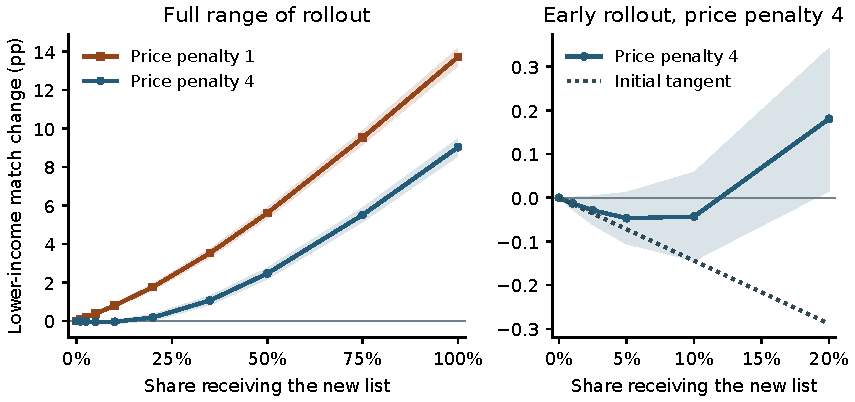
\includegraphics[width=.91\linewidth]{figures/rollout.pdf}
\caption{Partial rollout of the higher-income scoring rule in enriched five-listing markets. Shading gives pointwise 95\% block-bootstrap intervals. The dotted tangent is the exactly computed sum of the isolated effects at weight 4. The right panel enlarges early adoption.}
\label{fig:rollout}\Description{At score weight 4 the estimated gain is near zero early and rises to nine points by full adoption. The initial tangent is negative. At score weight 1 the effect is positive.}
\end{figure}

The experiment used 3,402,151 singleton insertions. On the first complete seed block 34,265 direct reruns checked singleton and score outcomes. Every realized baseline focal assignment agreed with the menu. The identities of matched lower-income renters agreed with residual-market DA for every score endpoint in every market. Switching editors in either forward or reverse order reproduced the final assignment and its total match change by summing successive, context-dependent changes. Separate exhaustive tests on 136,727 strict profiles across all labeled $2\times2$, $2\times3$, $3\times2$ and $3\times3$ feasible graphs checked the coalition identities and individual predictions. The archive also includes every market-level count used here.

\subsection{Does the scoring effect carry to another season?}
In the summer ordinary markets, holding rankings fixed at $(4,0.50)$ and varying only higher-income scoring weights $1,2,4$ gives lower-income spillovers of $+1.09,+0.49,-0.31$ points. A separate family of 36 simultaneous intervals excludes zero for each of those three comparisons. At a five-listing quota competitor-score changes can therefore reverse the effect on the fixed group even without changing rents or applicant tastes.

For a temporal check we fixed the January--March 2026 score comparison and its primary outcome before running this specific intervention. These months had been examined earlier under a simpler cheapest-first rule. They are fresh dates relative to summer calibration but not previously unseen catalogues. We froze summer quality, geography and price references and used the same calibration household pool. Using the calibrated cleaning rules across four boroughs gave 47,873 eligible winter records. We excluded 2,100 identifiable summer overlaps, 1,059 winter repeats and 24 ambiguous identities. All twelve winter cells supported both sampling designs. Eighty new blocks produced 1,920 markets and 11,520 DA outcomes. We also checked 288 entire assignment vectors against a second algorithm.

\begin{table}[t]\centering
\caption{Winter lower-income match rates, with each lower-income list fixed. The last column is the difference between the two scoring rules, with a simultaneous interval across twelve winter contrasts.}
\label{tab:winter}
\begin{tabular}{@{}llrrrr@{}}\toprule
Market draw & Quota & All uniform & Higher $T_1$ & Higher $T_4$ & $T_1-T_4$ (points)\\\midrule
Ordinary & Five & 3.07\% & 4.57\% & 2.56\% & $+2.01$ $[1.77,2.25]$\\
Ordinary & 40\% & 2.02\% & 3.19\% & 1.60\% & $+1.58$ $[1.32,1.84]$\\
Enriched & Five & 39.90\% & 53.08\% & 48.76\% & $+4.32$ $[3.92,4.72]$\\
Enriched & 40\% & 38.22\% & 43.70\% & 36.75\% & $+6.95$ $[6.52,7.38]$\\\bottomrule
\end{tabular}
\end{table}
The ordinary top-five spillover relative to uniform was $+1.50$ points at scoring weight 1 and $-0.51$ at weight 4. The preselected comparison \emph{between} scoring rules was $+2.01$ ($[1.85,2.18]$ pointwise). The result recurs in a different season with summer behavioral assumptions held fixed. The two seasons cannot establish how renters actually trade off price against other attributes.

\section{How much affordability does full stability permit?}\label{sec:burden}
Changing which renters match is one way to change a group's rent-burden distribution. Changing partners while keeping the recipients fixed is another. We compute the feasible improvement in that second comparison to see how much freedom remains once the platform promises stability.

Let the burden of an edge be $u_{bs}=12r_s/I_b$. The survey-weighted first quartile of contract-rent burden among recent lower-income movers with positive income, known rent and burden at most 40\% is 21.998\%. The cap excludes 33.10\% of otherwise eligible recent-mover survey weight. In the original 240 ordinary calibration markets ($20$ separate seed blocks), full DA with the fitted preferences placed 217 lower-income and 7,755 higher-income renter instances. Its lower-income first quartile of asking-rent burden was 31.21262\%. The 55th ordered burden is exactly the sample quartile since $1+(217-1)/4=55$. This target compares simulated advertised rents with contract rents in occupied homes.

\paragraph{The feasible supply bound.}
At burden threshold $t$ remove every edge whose burden exceeds $t$, restrict to lower-income applicants, and sum the maximum matching sizes across the disjoint market draws. Call the resulting count $K(t)$. Every allocation has at most $K(t)$ lower-income placements at this burden. At 21.998\% only two listing instances with any eligible edge qualify, against the required 55. The count reaches 55 for the first time at $27.77728\ldots\%$ and is 54 immediately below that value. A maximum cheap matching need not extend to 217 placements. Here an explicit matching of 55 cheap pairs extends by 713 disjoint eligible pairs. Keeping 162 of the additional pairs proves attainment at exactly 217. A second construction also attains this same floor while placing all 7,755 higher-income instances in aggregate. These bounds concern the finite sampled graphs.

\paragraph{An exact stable interval.}
Let $\mathcal S_m$ be the set of matchings stable on the complete feasible graph in market $m$. Matched-set invariance fixes the same group recipients in each market across $\mathcal S_m$. Write $c_t(M)$ for the number of designated-group recipients assigned burden at most $t$. For any integer order-statistic index $k$ the best and worst possible $k$th burden across stable allocations are respectively
\begin{align*}
 t_{\min}&=\min\{t:\sum_m \max_{M\in\mathcal S_m}c_t(M)\ge k\},\\
 t_{\max}&=\min\{t:\sum_m \min_{M\in\mathcal S_m}c_t(M)\ge k\}.
\end{align*}
Indeed, the local maxima can be attained simultaneously across distinct market draws. This characterizes when at least one global stable allocation has $k$ cheap placements. Using local minima characterizes when every global stable allocation has at least $k$. The count is linear in the edge indicators, so binary search over observed burdens and linear optimization on the integral stable-matching polytope give an exact algorithm \citep{rothblum1992polytope,gorski2009}. Minima of adjacent order statistics need not be simultaneously attainable; when the sample quartile interpolates, we evaluate the interpolated statistic on jointly attainable outcomes.

\begin{table}[t]\centering
\caption{Lower-income first-quartile asking-rent burden across the same 240 calibration markets. Counts and identities in the restrictions are those placed by full DA. The first four rows permit priority violations.}
\label{tab:welfare}
\begin{tabular}{@{}lr@{}}\toprule
Constraints & Lowest attainable quartile (\%)\\\midrule
Both income groups retain their pooled placement counts & 27.77728\\
Both groups retain their counts within every market & 28.13243\\
Every originally placed renter retains a placement & 28.37952\\
The same renters and listings remain occupied & 28.37952\\
Full-market stability & 31.21173\\\midrule
Renter-proposing DA (also the largest stable quartile) & 31.21262\\\bottomrule
\end{tabular}
\end{table}

Conditional on exactly the original matched renters and occupied listings, requiring stability raises the best quartile by \textbf{2.83221 percentage points}. Choosing a different stable matching can move the quartile by only \textbf{0.00089 points}. Of 240 markets, 86 admit multiple stable outcomes, yet only 3 of the 217 matched lower-income renter instances have more than one stable partner. The two differences answer different policy questions: the cost of requiring a stable allocation, and the choice available to a designer who retains that requirement.

We enumerated the 369 local stable outcomes (at most eight in any market), checking each for full-graph blocking pairs. An independent threshold linear program reproduced both stable endpoints. Feasible allocations attain every minimum in Table~\ref{tab:welfare}; fixed-volume matching or flow certificates exclude a lower value. Across the remaining eight calibration settings, we enumerated distinct jointly attainable burden vectors to evaluate interpolated quartiles directly (at most 12,288 combinations). The stable range of this quartile was at most 0.153 percentage points in all nine settings. Outcomes depend on modeled ordinal rankings, and lowering asking-rent burden need not be a Pareto improvement.

Expanding the inventory answers a separate supply question. With the same renters and 217 lower-income placements, the unrestricted pooled floor is 29.14\%, 27.78\%, 26.85\% and 25.29\% at 32, 64, 128 and 256 sampled listings per market. With the entire borough-month catalogue the pooled floor falls to 18.46\%, but preserving each market's original lower-income placement count puts it at 22.35\%, and preserving the original recipients yields 22.46\%. These last three bounds give lower-income renters first claim on all listings. Thirteen distinct listing records supply the feasible 21.998\%-burden edges across repeated whole-catalogue draws. Even its optimistic floor depends on which people and markets receive the placements; the advertised units may never all be available at once.

\section{Quota, information and interaction bounds}\label{app:menus}
\paragraph{A fixed quota.}
Order the $a=|A_h|$ attainable listings $j_1,\ldots,j_a$ by $h$'s preference. For $1\le k\le d$, a quota-$k$ list can deliver $j_r$ precisely when $r\le d-k+1$. Include $j_r$, exclude the $r-1$ better attainable listings, and fill the remaining $k-1$ slots from the other $d-r$ listings. Such a list can leave $h$ unmatched exactly when $k\le d-a$. A quota-respecting list matches $h$ without any loss to group $G$ iff at least one attainable $j_r$ satisfying the rank bound has $\ell(j_r)\notin G$. Choosing the highest-ranked such option gives $h$ their best assignment subject to this protection constraint. Under uniform sampling without replacement,
\[
  \Pr\{w(L)=j_r\}=\frac{\binom{d-r}{k-1}}{\binom{d}{k}},
  \qquad
  \Pr\{w(L)=\bot\}=\frac{\binom{d-a}{k}}{\binom{d}{k}},
\]
where an impossible binomial coefficient is zero. Weight the first probabilities by $\mathbf1\{\ell(j_r)\in G\}$ to obtain the exact group displacement probability. If $k=0$ or $d=0$, $h$ stays unmatched and no incumbent loses a match. At most $d+1$ DA runs identify every attainable listing and its label by comparing singleton entrants to the no-entry market. Each singleton can also be inserted by resuming the same completed no-entry DA state.

\paragraph{Sharp bounds.}
Incumbents $a,b$ have sole options $x,y$ respectively. Outsider $h$ is acceptable at $x,y,z$ and has top priority at each. With quota one, listing $z$ displaces nobody, $x$ displaces $a$ and $y$ displaces $b$. Changing $h$'s list from $x$ to $y$ costs one incumbent a match and gives another a match. Disjoint copies yield $m$ gains and $m$ losses from $m$ outsider list changes. These bounds are sharp on each margin. Change the $m$ lists sequentially and apply Corollary~\ref{cor:displacement} with everyone except the current editor fixed. Any pattern of protected versus unprotected labels on a focal applicant's ranked menu can be realized with a private incumbent at each listing and the focal applicant ranked first. The group effect has no universal sign.

Even with a common priority, the cardinality $|F(V)|$ can exhibit complementary and substitutable seats. Applicant $a$ ranks $y,x,z$, and $b$ accepts only $x$. All listings prioritize $a$ over $b$ whenever both are acceptable. Adding $y$ to $\{z\}$ adds no match, while adding $y$ to $\{x,z\}$ frees $x$ for $b$ and adds one. Adding $x$ to the empty market adds one match, while adding it to $\{z\}$ adds none. Thus $|F|$ is generally neither submodular nor supermodular.


\subsection{A short description of the externality}
For a platform wishing to answer many counterfactual reports, how much information about the rest of the market needs to be retained? The output determines the answer. Here the decoder must report which applicants are placed, allowing their partners to vary.

\begin{theorem}[Information needed to describe match status]\label{thm:status-bits}
Consider $n$ publicly labeled applicants, one of them focal, and $n$ publicly labeled unit-capacity listings. Other applicants' possibly incomplete preferences and the listing priorities can be preprocessed into a binary description. A decoder with only this description and the focal applicant's ordered report must return the matched/unmatched vector of all incumbents for every focal report. The optimal worst-case fixed-length description requires $\Theta(n\log n)$ bits. For every fixed nonempty group of incumbents, the optimal worst-case description of its matched count requires $\Theta(n)$ bits. The lower bounds hold under public common priorities fixed across the hard instances.
\end{theorem}
\begin{proof}
For the vector, encode the no-entry matched set in $n-1$ bits. At each listing encode one symbol: unattainable, attainable with no loss, or attainable displacing one named incumbent. There are at most $n+1$ symbols per listing. The decoder selects the best reported attainable listing and deletes its label, if any, from the no-entry set. Thus $n-1+n\lceil\log_2(n+1)\rceil$ bits suffice. For the group count store the baseline count and three symbols per listing: unattainable, attainable without a group loss, or attainable displacing a group member. This requires $O(n)$ bits.

For the vector lower bound give the focal applicant highest priority at every listing. Each of the $n-1$ other applicants accepts just one listing among the first $n-1$, in accordance with an arbitrary bijection between those applicants and those listings. A singleton focal report for listing $j$ makes exactly the incumbent paired to $j$ unmatched. The vector-valued response function recovers the entire bijection. The $(n-1)!$ distinct functions require at least $\log_2((n-1)!)=\Omega(n\log n)$ bits.

For the count, select $q$ in the specified group $G$. Give $q$ a single acceptable site $t$, and give every other incumbent $i$ a distinct private site $x_i$. Under a common priority, $h$ comes first and every nonmember of $G$ outranks $q$. For each of the $n-2$ incumbents $i\ne q$, choose an independent bit. A member of $G$ lists $x_i$ if its bit is one and otherwise submits an empty list. A nonmember ranks $x_i$ first and includes $t$ second exactly when its bit is one. Without the focal applicant, $q$ gets $t$. A singleton focal report for $x_i$ lowers the group count by exactly the bit at $i$. If $i$ is a member, it loses its own match. If $i$ is a nonmember, it can displace $q$ exactly when it listed $t$. The comparisons to the empty focal report recover all $n-2$ bits, giving $2^{n-2}$ different count functions. Unused sites complete the market to size $n$.
\end{proof}

This uses the report-to-output model of \citet{gtcomplexity}. They show that the complete DA partner-allocation function requires $\Omega(n^2)$ bits in the worst case (their Corollary 3.10). Theorem~\ref{thm:status-bits} concerns a coarser output with a sharp smaller bound. The bit counts describe the size of an offline representation available after the background market has been processed.


\begin{theorem}[Sharp interaction bound for one-slot recommendations]\label{thm:interaction}
Suppose each applicant sees at most one listing before and after the switch, and $h=|H|\ge2$. For $J=f(H)-f(\varnothing)-\sum_{i\in H}\delta_i$,
\[
                      -h \ \leq\ J\ \leq\ h-1+\lfloor h/2\rfloor .
\]
Both bounds are attained under a common strict priority.
\end{theorem}
\begin{proof}
At each listing keep only its highest-priority stationary applicant. It can contribute to $f$ only if this applicant is in $G$. An editor targeting that listing who outranks the stationary applicant is a threat. Discard listings with an unchanged threat. At any remaining listing write $d$ for the number of departing threats and $a$ for arriving threats. Under independent rollout its contribution to $\Phi(p)$ is $p^d(1-p)^a$: all departing threats must leave and no arriving threat can arrive. Subtracting its initial value and derivative from its final value gives $a-1$ if $d=0$ and $a\ge1$, $+1$ if $d\ge2$ and $a=0$, $-1$ if $d=1$ and $a\ge1$, and zero otherwise. There are at most $h$ additions and $h$ departures. The first positive contributions sum to at most $h-1$, the second to at most $\lfloor h/2\rfloor$, and the negative contributions total at least $-h$.

For the upper bound, arrange $\lfloor h/2\rfloor$ pairs of editors at separate origins (an extra singleton origin if $h$ is odd), all moving to one destination. Station a member of $G$ at every listing below all editors. For the lower bound, put one editor at each of $h$ listings and rotate all editors by one position. Switching one frees its origin, while joint rotation frees none. The universal bound concerns quota one; Proposition~\ref{prop:rollout}'s example survives padding at larger quotas.
\end{proof}

\section{Losses that a small rollout can miss}
\begin{theorem}[The limit of a low-saturation rollout]\label{thm:saturation-bound}
Fix $m$ outsiders, each with an old and a new shortlist, and any protected incumbent group $G$. Suppose every rollout involving at most $r$ outsiders preserves every initially matched member of $G$, where $0\le r\le m$. At most $m-r$ initially matched group members can lose their matches on full rollout. The bound is attained under a common listing priority, including a universal rule displaying $\min(k,d)$ whenever $k\ge r+1$.
\end{theorem}
\begin{proof}
Start with any $r$ changes. None of the initial matched group has been lost. Order the remaining $m-r$ changes arbitrarily. Apply Corollary~\ref{cor:displacement} to each current editor, treating all other applicants' lists as fixed. Each edit can cost at most one currently matched incumbent a match. Each final loser must have experienced such a transition at least once. The same upper bound needs only one lossless intermediate rollout of size $r$.

For sharpness, use core listings $x_1,\ldots,x_m$ and $m-r$ protected applicants. Incumbent $i$ lists the $r+1$ feasible cores $x_i,x_{i+1},\ldots,x_{i+r}$ in that order. Outsider $h_i$ has distinct private fallback $y_i$ and accepts its own core $x_i$. Give $h_i$ another $k-1$ private filler listings. Each filler has a dedicated applicant who lists it alone and outranks every outsider. Outsiders rank both meaningful options above their fillers. Every listing uses a strict common priority with dedicated applicants first, outsiders next, and incumbents last in increasing index order. Each outsider sees its $k-1$ fillers plus $y_i$ under its old list or $x_i$ under its new list. Every incumbent sees its entire list and every dedicated applicant sees its only choice.

Under a common priority, DA implements serial dictatorship in that priority order: the highest remaining applicant obtains their favorite remaining visible listing, and one repeats on the residual market. After at most $r$ switches, let $p_1<p_2<\cdots$ be the indices of unoccupied core listings after all outsiders have chosen. Among the first $i+r$ cores, at most $r$ are taken, so $i\le p_i\le i+r$. Inductively each protected incumbent $i$ gets $x_{p_i}$, its most preferred remaining core. At full rollout every core belongs to an outsider, so all $m-r$ previously matched protected applicants lose their match. For $r=1$ this already holds at a universal quota of two, and therefore at five under the displayed-size rule.
\end{proof}
With disjoint copies or additional isolated applicants, the construction applies to arbitrarily large markets. It demonstrates why a collection of lossless low-saturation tests can leave large losses unidentified at full rollout.


\section{Opening referrals after provisional offers}
Before allocation a recommendation changes exposure. After provisional offers an intermediary may have to reconcile full-market stability with promised ranks. Suppose each participant has a fixed representative and a paid audit opens every feasible edge incident to that representative's clients. Let $M_0$ be DA on the initial visibility graph and $M^+$ applicant-proposing DA under full visibility. Each applicant who prefers $M_0$ to $M^+$ must lose rank under every full-stable repair. For a protected group, a planner can spare every other member simultaneously by full disclosure. The \emph{protection premium} is the least cost of obtaining this guarantee with a globally stable DA outcome, minus the least cost of global stability alone. These actions and costs differ from the one-slot display edits studied before offers.

Theorems~\ref{thm:two} and~\ref{thm:three} give a sharp one-blocker boundary. If everyone has at most two acceptable partners and the provisional matching has at most one full-market blocker, every successful repair already protects the group. At degree three, for every odd $n=2m+1$ there is a connected market with one client per firm, unit costs, a perfect provisional assignment and exactly one blocker in which one audit repairs stability but protecting all applicants costs $m+1$. The mechanism is a rejection chain: opening one hidden offer gives the receiving side its favorite partners and moves all but one applicant below their original ranks. Protecting those ranks requires opening $m+1$ disjoint hidden opportunities. The appendix proves both results, gives the linear-time private-firm algorithm at degree two, and establishes hardness when a representative can serve multiple clients.

In a separately specified audit benchmark with independent listing lotteries, 40 blocks and four boroughs, lower-income protection cost nothing extra in all 480 markets under uniform top-five lists and under cheapest-first lists. Its donor split, catalogue cleaning and utility specification differ from the calibrated simulations. In one market, 15 audits made all edges of a full-stable allocation visible but all 4,096 minimum covers returned the same blocked DA outcome. Both ordinary and protected repair required 16 audits. A zero premium means a cheapest plan exists that meets the guarantee. It says little about how many applicants had an offer to protect.

\section{Repairing a provisional assignment}\label{sec:repair}
Let $B$ and $S$ be finite sets of applicants and listings. Each vertex has capacity one and strictly ranks its neighbors in a bipartite graph $E\subseteq B\times S$ above being unmatched, denoted by $\bot$. Write $M(i)$ for the partner of $i$ in a matching $M$. A pair $bs\in E$ blocks if $s\succ_b M(b)$ and $b\succ_s M(s)$. Full stability means no such pair exists. DA on a graph $H$ restricts each ranking to its neighbors in $H$. Rejected applicants propose to their next visible choice. We use applicant-proposing DA unless otherwise stated.

Let $E_0\subseteq E$ be the graph of initial shortlists and $M_0=\da(E_0)$. Participant $i$ belongs to firm $f(i)$, whose audit costs a positive integer $c_{f(i)}$. For a set $A$ of audited firms, put
\[
 H(A)=E_0\cup\{bs\in E: f(b)\in A\text{ or } f(s)\in A\}.
\]
A plan succeeds if $D(A)=\da(H(A))$ is stable on $E$. Write $c(A)=\sum_{f\in A} c_f$ and let $\co$ be the least cost of success. A successful outcome may differ from full disclosure. The institution can change exposure but must honor its allocation rule.

Let $M^+$ and $M^-$ denote applicant- and listing-proposing DA on $E$. Every full-stable matching assigns each applicant a partner weakly between these two extremes \cite{gale1962,roth1986}. For a protected group $G\subseteq B$ define
\[
 \HH(M)=\{b\in G:M_0(b)\succ_b M(b)\}.
\]
Write $F_G=\HH(M^+)$. Every successful repair incurs all losses in $F_G$. Opening all firms attains exactly $F_G$. We define $C_G$ as the least cost of a successful plan with $\HH(D(A))=F_G$ and $\Delta_G=C_G-\co$. This criterion counts people experiencing a strict loss. The size of a loss within $F_G$ can still depend on the chosen repair. Initially unmatched applicants automatically clear their threshold.

\begin{proposition}[Two-run certificate]\label{prop:screen}
If no $b\in G$ satisfies $M^+(b)\succeq_b M_0(b)\succ_b M^-(b)$, every successful plan meets the group's protection requirement and $\Delta_G=0$.
\end{proposition}
\begin{proof}
Each $b\in G\setminus F_G$ then weakly prefers even their worst full-stable assignment to $M_0(b)$. Apply the extremal bounds to the response of any successful plan.
\end{proof}
A renter whose threshold falls between the extremes makes the test inconclusive. The cheapest ordinary plan may already give that renter a sufficiently good partner.

\subsection{A boundary at two acceptable partners}
The next result applies to arbitrary positive costs and any distribution of clients among firms. Degree always refers to the number of acceptable partners in $E$, on \emph{both} sides.

\begin{theorem}[One blocker at degree two]\label{thm:two}
At maximum degree two, every successful plan attains $F_G$ for every $G$ if $M_0$ has at most one full-market blocker. The same conclusion holds for any perfect $M_0$.
\end{theorem}
\begin{proof}
A connected component of $E$ is a path, a cycle, or an isolated vertex. All stable matchings have the same matched participants \cite{roth1986}, so two stable matchings can differ only along alternating cycles. At degree two an alternating cycle takes up its entire component. Hence a component with more than one stable outcome is an even cycle with exactly two stable perfect matchings. Denote its applicant-optimal alternation by $P$ and its other alternation by $Q$. Every applicant prefers their $P$ edge because their partners differ. Each listing prefers its $Q$ edge since otherwise its $P$ edge would block $Q$.

Consider any partial matching on such a cycle. A $P$ edge blocks exactly when its listing is unmatched: if matched along $Q$, that listing holds its favorite applicant. Likewise a $Q$ edge blocks exactly when its applicant is unmatched. With $k$ unmatched participants on each side there are therefore exactly $2k$ blocking pairs. If the entire market has at most one blocker, every cycle admitting a choice of stable outcomes is already perfectly matched in $M_0$.

On each such cycle $M_0$ uses $P$ or $Q$. If it uses $P$, the applicants' distinct first choices are visible in every expansion, so DA always returns them. If it uses $Q$, both stable outcomes weakly improve on every applicant's initial partner. On a component with a unique stable matching all losses are fixed. This also proves the claim for a perfect $M_0$, regardless of the number of initial blockers elsewhere.
\end{proof}

\paragraph{Sharpness with a vacancy.}
For $n\geq3$, take indices modulo $n$. Applicant $a_i$ ranks $s_i$ then $s_{i+1}$, and $s_j$ ranks $a_{j-1}$ then $a_j$. Each person has a private firm of unit cost. Initially expose $a_0s_0$ and all one-step edges $a_i s_{i+1}$ except $a_{n-1}s_0$. There is one unmatched participant on each side, and precisely two blockers by the counting identity. Auditing $s_0$ gives every listing its favorite and costs one. Protecting $a_0$ requires the diagonal matching since it is the only stable matching containing $a_0s_0$. Its $n-1$ other edges are hidden and disjoint, so each needs a separate audit. Auditing their applicants attains this cost. Thus two blockers suffice for an unbounded premium at degree two.

\begin{theorem}[One blocker at degree three]\label{thm:three}
For every odd $n=2m+1\geq3$ there is a connected market with $n$ participants on each side, degree three everywhere, private unit-cost firms, a perfect initial matching and exactly one blocking pair, in which $\co=1$ and $\allp=m+1$.
\end{theorem}

\begin{table}[t]
\centering
\begin{tabular}{@{}lrrrrrrr@{}}\toprule
Applicant $i$ & 0&1&2&3&4&5&6\\ \midrule
Initial partner        &0&1&2&3&4&5&6\\
One-audit repair       &1&2&3&4&5&6&0\\
Four-audit repair      &1&3&2&5&4&0&6\\
Full disclosure        &2&3&4&5&6&0&1\\ \bottomrule
\end{tabular}
\caption{The seven-applicant example. Entries are listing indices. In the one-audit row applicants 1 through 6 fall from second to last choice. In the four-audit row applicants 1, 3 and 5 get their first choices, 2, 4 and 6 keep their partners, and 0 improves.}
\label{tab:ring}
\end{table}

\begin{proof}
Take indices modulo $n$. Each $a_i$ finds listings $s_i,s_{i+1},s_{i+2}$ acceptable. Rankings from best to worst are
\[
\begin{array}{c@{\quad}lll}
 a_0 & s_2 & s_1 & s_0\\
 a_i\ (i>0)& s_{i+2}&s_i&s_{i+1}\\
 s_j & a_{j-1}&a_j&a_{j-2}.
\end{array}
\]
Expose all diagonal and one-step edges except $a_0s_1$. Initially all applicants obtain the diagonal. A two-step target prefers its diagonal holder. Only $a_0$ prefers its one-step target to its diagonal, and $s_1$ prefers $a_0$. Thus $a_0s_1$ is the sole blocker. In the full market the applicants' two-step first choices are all distinct, so $F_B$ is empty.

Audit listing $s_1$. It accepts $a_0$ and rejects $a_{n-1}$ on the other newly visible edge. The displaced $a_1$ takes $s_2$, displacing $a_2$, and the chain continues around the cycle. Every listing obtains its first choice. Zero audits leave a blocker, so $\co=1$.

Any full-stable response is perfect by matched-set invariance. To protect everyone, positive-index applicants may use only their diagonal or two-step edges. If $a_0$ uses one of those edge types as well, the perfect matching must be all diagonal or all two-step: the permutation $i\mapsto i+2$ is one cycle for odd $n$. The diagonal is unstable, and the all-two-step matching needs all $n$ hidden, disjoint edges. If $a_0$ uses $s_1$, it forces $a_1$ onto $s_3$, then $a_3$ onto $s_5$, through $a_{2m-1}$ onto $s_0$. These $m$ two-step edges and $a_0s_1$ are hidden and disjoint, requiring at least $m+1$ audits.

Audit $s_1$ and the $m$ odd-indexed applicants. The latter get their two-step first choices. Applicant $a_0$ gets $s_1$ and each positive even applicant keeps its diagonal (the extra proposal to $s_1$ is rejected). Only $a_0$ and the positive even applicants could prefer another listing. Their two-step targets hold their diagonal applicant or their favorite at $s_1$. None blocks. This attains the lower bound and gives Table~\ref{tab:ring} for $n=7$.
\end{proof}

\paragraph{A five-listing rule.}
The example also works if everyone must see $\min(5,d)$ of their $d$ acceptable listings. Give each core applicant four additional, lower-ranked listings, each with a dedicated applicant. A filler and its dedicated applicant rank each other first and always see one another. Show $a_0$ all four fillers and every other core applicant three. The additional pairs can never prevent or displace a core match. The cost result survives, with core applicant degree now seven.

\subsection{Computing the protection premium}
\begin{theorem}[Private firms at degree two]\label{thm:linear}
With one client per firm and maximum degree two, $\co$ and $C_G$ and attaining plans can be computed in linear time in the explicit market size, counting arithmetic operations.
\end{theorem}
\begin{proof}
Fix any expanded graph $H$ containing a full-stable matching $M$. The restriction of $M$ is stable on $H$. On a forest component of $H$ it is the unique stable assignment, since two stable assignments would differ along a cycle. Any cycle component of $H$ is an intact component of $E$. There DA is full-stable already. Every hidden edge has endpoints outside intact cycles, where DA agrees with $M$, so no hidden edge blocks. Further, applicant-optimality on $H$ transfers any applicant rank thresholds from $M$ to $\da(H)$. Thus exposing a qualifying full-stable matching is necessary and sufficient at degree two, even with shared firms.

Compute $M_0,M^+,M^-$. On each full component the latter two enumerate its one or two stable outcomes. Discard those that breach a protected threshold outside $F_G$. For each remaining local matching $M$, its least exposure cost is
\[
       w(M)=\sum_{bs\in M\setminus E_0}\min\{c_{f(b)},c_{f(s)}\}.
\]
The hidden matching edges are disjoint and each client has its own firm. Buying the cheaper endpoint of each edge is sufficient and necessary in sum. Choose the least costly qualifying matching per component. Omitting all thresholds gives $\co$. Three DA runs and a constant number of graph scans take linear time.
\end{proof}

\paragraph{Shared portfolios.}
The budget decision for either cost becomes NP-complete even with unit costs, at most three clients per firm and two choices per person. Reduce from vertex cover on a cubic graph \cite{alimonti2000}. Give each vertex a firm. An edge with endpoints $u,v$ creates an isolated two-by-two market with applicants $p,q$ represented by $u,v$, respectively, and listings $x,y$, each with a private firm. Let $p$ rank $y,x$, $q$ rank $x,y$, $x$ rank $p,q$ and $y$ rank $q,p$. Initially only $px,qx$ are open and $p$ takes $x$. With neither endpoint nor $y$ audited, $q$ and $y$ block. Auditing $u$ or $y$ yields $py,qx$, giving both applicants first choices. Auditing $v$ alone yields $px,qy$, giving both listings first choices. Both outcomes protect every applicant. Thus each edge requires one of $u,v,y$. Replace each audited private $y$ by an endpoint and discard $x$ audits to obtain a vertex cover of no greater cost. Conversely every cover is a successful protected plan of the same cost. Full DA, restricted DA and a full blocking check verify a budget certificate in polynomial time. The same cost-preserving reduction gives APX-hardness of both minimizations. The hard choice here is which representatives to open. Running DA itself takes polynomial time.

\paragraph{General markets.}
Choose binary firm variables $x_f$ and impose $y_e=1$ for $e\in E_0$. Else impose the logical OR of the endpoint audits, $y_e\geq x_{f(b)},x_{f(s)}$ and $y_e\leq x_{f(b)}+x_{f(s)}$, with $0\le y_e\le1$. Minimize $\sum_f c_fx_f$. To certify a stable matching can be supported, use nonnegative variables $z_e\le y_e$ with incident sums at most one and a stability inequality for each $bs\in E$:
\[
 z_{bs}+\sum_{t\succ_b s}z_{bt}+\sum_{a\succ_s b}z_{as}\ \geq\ 1 .
\]
For each initially matched $b\in G\setminus F_G$ also impose
\begin{equation}
        \sum_{s\succeq_b M_0(b)}z_{bs}=1. \label{eq:rank}
\end{equation}
For fixed integer audits the support restrictions set coordinates to zero. Each rank row saturates a valid upper bound. Together they select a face of the integral stable-matching polytope \cite{rothblum1992polytope}. Thus a feasible master solution guarantees an integral stable witness meeting the thresholds. It is stable on the visible graph, where proposer DA weakly dominates it. This proves that the DA response meets the thresholds. In degree three or higher a hidden pair can still block that response.

We rerun DA on each candidate and check every full edge. For a connected component of $E$ containing a blocker, let $P$ contain every applicant's feasible edges weakly above their final partner in this run (all their edges if unmatched). Keep the visibility status of every edge in $P$ fixed and rerun the same proposal schedule. Induction on proposals gives exactly the same proposals and rejections in that component: nobody reached a lower-ranked edge in the original run. To exclude all repetitions of that failure, require
\[
   \sum_{e\in P:\,y_e^*=1}(1-y_e)+
   \sum_{e\in P:\,y_e^*=0}y_e\ \geq\ 1 ,
\]
where $y^*$ denotes the failed exposure. The constraint removes at least the current plan and preserves every successful one. There are finitely many plans and full disclosure is feasible. A successful protected response is itself a master witness, so the optimum of the master lower-bounds the plan cost throughout. Matching it with a verified incumbent certifies optimality.

\paragraph{Computational check.}
We solved 160 synthetic markets with 24 participants per side and ten unit-cost firms, crossing one or four local markets, independent or correlated rankings, and 25\% or 50\% mean exposure (20 paired seeds). Simulated partnerships quadruple exposure odds and half of applicants receive an odds multiplier of one half. Both solvers start from the same protected reverse-deletion plan and use one HiGHS thread, a 15-second limit and the same DA checks. Including the threshold rows in Equation~(\ref{eq:rank}) reduced master calls from 195 to 163 on the first paired run, and median time from 48.2 to 32.1\,ms across three repeats. Both methods certified all optima against enumeration. Protection cost one additional audit in six markets and zero extra in 154. In a separate exhaustive test, the degree-two formula agreed with optimization in 475,352 weighted group cases on three-by-three graphs.


\section{Further controls for exposure and competition}
The main calibrated results use a change exclusively to higher-income recommendations. A joint switch for both income groups is a different policy. In the initial 20-block enriched five-listing pilot the lower-income match rate rose from 36.38\% to 45.13\% when only the higher group switched to $T_4$. When both groups switched, the rate was 19.23\%. Endpoint accounting assigns $+10.95$ points to net transfers of occupied listings between income groups and $-2.20$ points to transitions involving vacancies under the higher-only switch. Of 2,790 lower-income instances shown their entire nonempty list, 65 lost a match and 41 gained one. In the ordinary pilot, changing only higher-income lists reduced the lower-income match rate by 0.38 points. These studies share the summer catalogues.

\paragraph{Sensitivity to preferences.}
On the 100 fresh summer blocks, varying the transparent score and the latent renter model together gave the results in Figure~\ref{fig:grid}. At fitted preferences the proportional quota gave lower-income spillovers of $-0.26$ and $-1.33$ points in ordinary and enriched markets. Enriched top-five effects were positive across all nine parameters, while ordinary top-five effects were positive at six and negative at three. The primary and exploratory price-crossing grids used 129,600 DA allocations each on an NVIDIA H200, with complete counts reproduced by an independent sequential implementation. The two grids reuse markets. Primary-grid uncertainty uses 10,000 paired blocks resamples and a simultaneous maximum standardized deviation over 36 contrasts.
\begin{figure}[ht]\centering
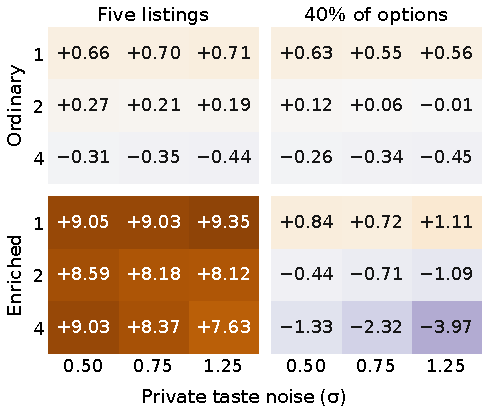
\includegraphics[width=.6\linewidth]{figures/preference_grid.pdf}
\caption{Fresh-block higher-income-only score spillovers (points). Rows within a panel are latent and scoring price weights 1, 2, 4; columns are private taste noise. Ordinary top-five is sensitive to the price assumption.}
\label{fig:grid}\Description{Four three-by-three panels giving signed effects. All enriched top-five cells have positive estimates, while other panels vary.}
\end{figure}

\paragraph{Which part of enrichment matters?}
On 40 further blocks we separately varied the listing draw and the renter-selection rule. Across 408 cell--seed combinations supporting all four arms, the five-listing spillover was $-0.44$ points using ordinary listings and ordinary renters, and $+3.48$ with band listings and the same renters. The paired difference was $+3.92$ ($[3.20,4.70]$). With selected renters these effects were $-0.79$ and $+8.92$. The 72 other ordinary catalogues admitted no eligible lower-income donor for the selected-renter arm. The four-way comparison conditions on common support. The ordinary main comparison includes those scarce markets.

\paragraph{A fixed-quota capacity control.}
Let $\nu(E)$ be full-graph maximum matching cardinality. Among assignments of size $\nu(E)$ choose one with the fewest undisplayed matched pairs; break ties by total observable rank. Its hidden edges are a lower bound on the edits needed to show any such assignment. The bound is attained by replacing each affected renter's worst displayed option with their witness edge, since the witness matches each renter at most once. The rule assumes each renter with eligible options has at least one slot. In the enriched five-listing pilot this changed 11.09\% of slots: visible capacity rose from 24.74 to 55.54 placements per market; DA placements rose from 23.44 to 44.39. The lower-group match rate was 47.58\% against 28.35\% when the same removed slots were randomly replaced, and 36.38\% under uniform lists. Every repaired market still had a full-graph blocker. Archive results include both quotas and market designs.

\paragraph{Verification scope.}
The package includes the summer and winter cohort rules and block-level counts, replay scripts, exact assignments and lower bounds, parameter grids and study designs. The pricing crossover, individual-displacement and stable-quartile analyses are follow-ups to the earlier calibrated results. Different experiments reuse survey households. The winter study evaluates a previously untested scoring intervention on a cohort that had been used for a simpler policy. None of the experiments measures field behavior or validates model-based welfare against outcomes of actual leases.

\end{document}
